
\documentclass[12pt,twoside]{book}

\usepackage[a4paper,top=2.2cm,bottom=2.3cm,left=2.2cm,right=2.2cm]{geometry}
\usepackage{graphicx}
\usepackage{booktabs}
\usepackage{longtable}
\usepackage{array}
\usepackage{tabularx}
\usepackage{enumitem}
\usepackage{xcolor}
\usepackage{listings}
\usepackage{fancyhdr}
\usepackage{hyperref}
\usepackage{bookmark}
\usepackage{tikz}
\usetikzlibrary{arrows.meta,positioning,shapes.geometric,fit,calc}
\usepackage[most]{tcolorbox}
\usepackage{setspace}
\usepackage{multicol}
\usepackage{amssymb}
\usepackage{amsmath}
\usepackage{xepersian}

\settextfont[AutoFakeSlant=0.18]{Vazirmatn}
\setlength{\emergencystretch}{1.5em}
\setlatintextfont{DejaVu Sans}
\setmonofont{DejaVu Sans Mono}
\setdigitfont{Vazirmatn}

\definecolor{Ink}{HTML}{12162B}
\definecolor{InkSoft}{HTML}{1B2140}
\definecolor{Parchment}{HTML}{F5F1E6}
\definecolor{Spark}{HTML}{F2A93B}
\definecolor{Tide}{HTML}{3E8C8C}
\definecolor{Ember}{HTML}{E1573A}
\definecolor{Ash}{HTML}{666A78}
\definecolor{CodeBg}{HTML}{F4F5F7}
\definecolor{DecisionBg}{HTML}{FFF7E8}
\definecolor{SourceBg}{HTML}{EEF7F7}
\definecolor{WarningBg}{HTML}{FFF0ED}

\hypersetup{
  colorlinks=true,
  linkcolor=InkSoft,
  urlcolor=Tide,
  citecolor=InkSoft,
  pdftitle={InsightInk Developer Bible},
  pdfauthor={InsightInk Project}
}

\setlength{\parindent}{0pt}
\setlength{\parskip}{0.55em}
\setlist[itemize]{topsep=0.25em,itemsep=0.2em,parsep=0em}
\setlist[enumerate]{topsep=0.25em,itemsep=0.2em,parsep=0em}
\renewcommand{\arraystretch}{1.35}
\onehalfspacing

\pagestyle{fancy}
\fancyhf{}
\fancyhead[LE,RO]{\small راهنمای جامع توسعه InsightInk}
\fancyhead[RE,LO]{\small \leftmark}
\fancyfoot[C]{\thepage}
\setlength{\headheight}{15pt}

\newcommand{\tech}[1]{\lr{\texttt{\detokenize{#1}}}}
\newcommand{\eng}[1]{\lr{#1}}
\newcommand{\filepath}[1]{\lr{\texttt{\detokenize{#1}}}}
\newcommand{\http}[1]{\lr{\texttt{\detokenize{#1}}}}
\newcommand{\term}[1]{\textbf{#1}}

\newtcolorbox{decisionbox}[1][]{
  colback=DecisionBg,
  colframe=Spark!75!black,
  title={تصمیم پروژه},
  fonttitle=\bfseries,
  breakable,
  #1
}

\newtcolorbox{sourcebox}[1][]{
  colback=SourceBg,
  colframe=Tide!80!black,
  title={برگرفته از نیازمندی‌های منبع},
  fonttitle=\bfseries,
  breakable,
  #1
}

\newtcolorbox{learningbox}[1][]{
  colback=CodeBg,
  colframe=InkSoft!70,
  title={چیزی که باید یاد بگیری},
  fonttitle=\bfseries,
  breakable,
  #1
}

\newtcolorbox{warningbox}[1][]{
  colback=WarningBg,
  colframe=Ember!80!black,
  title={هشدار / دام رایج},
  fonttitle=\bfseries,
  breakable,
  #1
}

\newtcolorbox{donebox}[1][]{
  colback=green!4,
  colframe=green!45!black,
  title={معیار پایان این مرحله},
  fonttitle=\bfseries,
  breakable,
  #1
}

\lstdefinestyle{code}{
  backgroundcolor=\color{CodeBg},
  basicstyle=\ttfamily\small,
  frame=single,
  rulecolor=\color{Ash!30},
  breaklines=true,
  showstringspaces=false,
  tabsize=2,
  numbers=left,
  numberstyle=\tiny\color{Ash},
  xleftmargin=1.5em,
  framexleftmargin=1em
}
\lstset{style=code}

\newcommand{\codeblock}[1]{%
\begin{latin}
\begin{lstlisting}
#1
\end{lstlisting}
\end{latin}
}

\newcommand{\phase}[1]{\subsection*{فاز #1}}


\begin{document}

\frontmatter
\begin{titlepage}
\centering
\vspace*{3cm}
{\Huge\bfseries \eng{InsightInk}\par}
\vspace{0.7cm}
{\Large\bfseries راهنمای جامع معماری، یادگیری و توسعه\par}
\vspace{0.4cm}
{\large \eng{Developer Bible}\par}
\vfill
{\large پروژه کارشناسی\par}
\vspace{0.5cm}
{\large نسخه برنامه‌ریزی اولیه -- آبان ۱۴۰۵ / اکتبر ۲۰۲۶\par}
\vspace*{2cm}
\end{titlepage}

\begin{tcolorbox}[colback=Parchment,colframe=InkSoft,title={وضعیت سند},fonttitle=\bfseries]
این سند نقشه اصلی توسعه پروژه \eng{InsightInk} است. هدف آن این است که توسعه‌دهنده بتواند حتی بدون دسترسی به ابزارهای هوش مصنوعی، مسیر پروژه را از مرحله آماده‌سازی محیط تا پیاده‌سازی، تست، استقرار و مستندسازی دانشگاهی ادامه دهد.

نسخه‌های محلی تأییدشده هنگام نگارش:
\begin{itemize}
  \item \eng{Python 3.14.8}
  \item \eng{Django 5.2.18}
  \item سیستم توسعه: \eng{Linux / PyCharm / Git}
\end{itemize}

این سند بین سه نوع اطلاعات تفکیک می‌کند:
\begin{enumerate}
  \item نیازمندی‌های مستقیم استخراج‌شده از \eng{PDS}، بردهای \eng{Epic/User Story/NFR/WSJF} و پروتوتایپ؛
  \item تصمیم‌های معماری و محدودسازی دامنه که بعداً برای پروژه کارشناسی گرفته شده‌اند؛
  \item پیشنهادهای فنی و آموزشی که برای اجرای قابل‌فهم و قابل‌دفاع پروژه اضافه شده‌اند.
\end{enumerate}
\end{tcolorbox}

\tableofcontents
\clearpage

\chapter*{چگونه از این سند استفاده کنیم}
\addcontentsline{toc}{chapter}{چگونه از این سند استفاده کنیم}

این سند قرار نیست فقط خوانده شود. در طول توسعه باید نقش چک‌لیست و مرجع روزمره را داشته باشد.

چرخه پیشنهادی هر مرحله:
\[
\text{یادگیری} \rightarrow \text{فهم} \rightarrow \text{پیاده‌سازی} \rightarrow \text{تست} \rightarrow \text{مستندسازی} \rightarrow \text{Commit}
\]

اگر در هر مرحله نتوانی توضیح بدهی یک ابزار چه مشکلی را حل می‌کند، چرا به پروژه اضافه شده، چه داده‌ای می‌گیرد و چه خروجی‌ای می‌دهد، هنوز زمان عبور از آن مرحله نیست.

\mainmatter


\chapter{معرفی محصول و مسئله}

\section{InsightInk چیست؟}

\eng{InsightInk} یک سامانه محتوایی است که ایده‌های مفید استخراج‌شده از کتاب، مقاله، فیلم/مستند و پادکست را در قالب یک Feed در اختیار کاربر قرار می‌دهد. ایده اصلی محصول این است که «اسکرول کردن» به‌جای مصرف محتوای صرفاً سرگرم‌کننده، به مواجهه با تجربه‌ها و ایده‌های قابل‌فکر و قابل‌عمل تبدیل شود.

\begin{sourcebox}
در PDS، محصول به‌عنوان فضایی برای مرور ایده‌های حاصل از تجربه خواندن کتاب و مقاله، دیدن فیلم و شنیدن پادکست معرفی شده است. کاربر می‌تواند از این محتوا الهام بگیرد، آن را ذخیره یا به اشتراک بگذارد و با سازندگان محتوا ارتباط بگیرد.
\end{sourcebox}

\section{هدف این پروژه دانشگاهی}

هدف ما ساخت یک استارتاپ production در مقیاس میلیون‌ها کاربر نیست. هدف عبارت است از:

\begin{itemize}
  \item ساخت یک پروژه Full-Stack واقعی و قابل اجرا؛
  \item یادگیری عمیق \eng{Python} و \eng{Django}؛
  \item یادگیری Frontend از مبانی تا \eng{React + TypeScript}؛
  \item طراحی درست دیتابیس رابطه‌ای؛
  \item ساخت API، احراز هویت، Permission و تست؛
  \item پیاده‌سازی سیستم پیشنهاددهی الگوریتمی قابل توضیح؛
  \item پشتیبانی هم‌زمان از فارسی و انگلیسی؛
  \item داشتن مستندات کامل برای ادامه کار بدون وابستگی به AI.
\end{itemize}

\begin{decisionbox}
معماری باید برای یک نفر قابل نگهداری باشد. بنابراین \eng{microservice}، \eng{Kubernetes}، \eng{event bus}، \eng{vector database} و زیرساخت‌های سنگین وارد Baseline نمی‌شوند.
\end{decisionbox}

\section{Actorهای اصلی}

\subsection{Reader / User}

کاربر معمولی که می‌تواند:
\begin{itemize}
  \item ایده‌ها را بخواند؛
  \item Spark بزند؛
  \item ذخیره کند؛
  \item نظر بدهد؛
  \item Creator را Follow کند؛
  \item ایده‌ها را جست‌وجو کند؛
  \item کتابخانه شخصی داشته باشد؛
  \item محتوای نامناسب را Report کند؛
  \item در فاز پیام‌رسانی با Creator تماس بگیرد.
\end{itemize}

\subsection{Creator}

Creator یک User جداگانه از نظر هویتی نیست؛ یک User است که \eng{CreatorProfile} و Permissionهای مربوط را دارد. او می‌تواند پروفایل سازنده داشته باشد، محتوای خودش را منتشر/مدیریت کند و با مخاطب تعامل داشته باشد.

\subsection{Moderator}

Moderator ناظر سیستم است و دسترسی‌های محدود اما قوی برای Trust \& Safety دارد:
\begin{itemize}
  \item مشاهده Reportها؛
  \item بررسی محتوای گزارش‌شده؛
  \item مخفی/حذف کردن Comment یا Content طبق سیاست؛
  \item ثبت اقدام Moderation؛
  \item اعمال محدودیت‌های مشخص روی User در صورت نیاز.
\end{itemize}

Moderator مدیر کل نیست و اجازه ایجاد Moderator یا Admin ندارد.

\subsection{Admin}

Admin مدیر کل سیستم است و بالاترین دسترسی را دارد. فقط Admin می‌تواند Moderatorها را تعیین یا حذف کند.

\section{زبان‌های محصول}

\begin{decisionbox}
زبان اصلی محصول فارسی و زبان دوم انگلیسی است. از روز اول ساختار Frontend و مدل داده باید امکان \eng{RTL/LTR} و محتوای دو زبانه را در نظر بگیرد.
\end{decisionbox}

این یعنی:
\begin{itemize}
  \item UI فارسی راست‌به‌چپ؛
  \item UI انگلیسی چپ‌به‌راست؛
  \item زبان UI از زبان Content جداست؛
  \item کاربر می‌تواند UI فارسی داشته باشد و محتوای انگلیسی ببیند.
\end{itemize}

\section{تعریف AI در این پروژه}

\begin{warningbox}
در منابع اولیه عباراتی مانند \eng{AI-Assisted Tool} و \eng{AI-Powered Idea Discovery} آمده است. در Scope نهایی این پروژه، هیچ LLM یا RAG یا Agent وجود ندارد.
\end{warningbox}

سیستم پیشنهاددهی ما کاملاً الگوریتمی است و با داده‌هایی مانند Interest، Save، Spark، Follow، تازگی محتوا و Popularity کار می‌کند.

مواردی که صریحاً خارج از پروژه هستند:
\begin{itemize}
  \item \eng{OpenAI/Claude/Gemini API}
  \item \eng{LLM}
  \item \eng{RAG}
  \item \eng{Embeddings}
  \item \eng{Vector DB}
  \item \eng{Prompt Engineering}
  \item \eng{AI Agent}
\end{itemize}

\section{معیار موفقیت پروژه}

در پایان، پروژه باید حداقل بتواند Flow زیر را واقعاً اجرا کند:

\begin{enumerate}
  \item کاربر Account بسازد و Login کند؛
  \item زبان و علاقه‌مندی‌ها را انتخاب کند؛
  \item Feed واقعی از PostgreSQL ببیند؛
  \item Idea را باز کند؛
  \item Source آن را ببیند؛
  \item Spark/Save/Comment کند؛
  \item Saved Ideaها را در Library ببیند؛
  \item Creator را ببیند و Follow کند؛
  \item Search/Explore داشته باشد؛
  \item Recommendation الگوریتمی دریافت کند؛
  \item UI فارسی و انگلیسی درست داشته باشد.
\end{enumerate}

Realtime، Messaging، Notification، TTS و Membership/eBook بعد از این Core Flow اضافه می‌شوند.


\chapter{دامنه پروژه و نیازمندی‌ها}

\section{منابع نیازمندی}

مبنای این سند مجموعه فایل‌های پروژه است:
\begin{itemize}
  \item \eng{PDS.pdf}
  \item بردهای \eng{Epic / Feature / User Story}
  \item برد \eng{Non-Functional Requirements}
  \item برد \eng{WSJF Prioritization}
  \item پروتوتایپ \eng{InsightInk Investor Prototype}
\end{itemize}

پروتوتایپ به‌عنوان مرجع Flow، Design Language و Screenها استفاده می‌شود، نه Codebase production.

\section{قابلیت‌های اصلی برگرفته از PDS}

\begin{sourcebox}
PDS قابلیت‌های زیر را مشخص می‌کند:
\begin{itemize}
  \item خواندن یا Share کردن تجربه مرتبط با کتاب، مقاله، فیلم یا پادکست؛
  \item Save، Share و Comment روی Idea؛
  \item Pagination؛
  \item Estimated Reading Time؛
  \item Text-To-Speech؛
  \item Idea Suggesting و Idea Exploring Algorithm؛
  \item Library، eBook و Membership؛
  \item ارتباط مستقیم با Writer/Director/Podcast Maker؛
  \item SQL relational database، CDN و real-time sync.
\end{itemize}
\end{sourcebox}

\section{نه Epic اصلی}

\begin{enumerate}
  \item \eng{AI-Powered Idea Discovery}
  \item \eng{Real-Time, Cross-Device Experience}
  \item \eng{Creator Direct-Access Network}
  \item \eng{Library Membership \& eBooks}
  \item \eng{Core Idea Feed \& Multi-Format Content}
  \item \eng{Onboarding \& Account Setup}
  \item \eng{Engagement \& Social Signals}
  \item \eng{Multimodal Access (Text-to-Speech)}
  \item \eng{Notifications \& Activity Awareness}
\end{enumerate}

\section{تفکیک Scope نهایی}

\subsection{Core MVP}

Core MVP باید شامل این موارد باشد:
\begin{itemize}
  \item Register/Login؛
  \item Profile؛
  \item انتخاب Interest؛
  \item Topic/Source/Idea/Creator data model؛
  \item Feed با Pagination؛
  \item Idea Detail؛
  \item Search/Explore؛
  \item Spark؛
  \item Save/Library؛
  \item Comment؛
  \item Creator Profile؛
  \item Follow؛
  \item Report پایه؛
  \item Recommendation الگوریتمی؛
  \item فارسی/انگلیسی و RTL/LTR.
\end{itemize}

\subsection{فاز دوم}

بعد از Core:
\begin{itemize}
  \item Realtime Sync؛
  \item Direct Messaging؛
  \item Notifications؛
  \item TTS؛
  \item Membership/eBooks؛
  \item Offline behavior در حدی که واقعاً قابل انجام و قابل تست باشد.
\end{itemize}

\subsection{موارد خارج از Scope}

\begin{itemize}
  \item Generative AI؛
  \item RAG؛
  \item Embedding؛
  \item Agent؛
  \item Microservice؛
  \item Native mobile codebase جدا؛
  \item ذخیره اطلاعات کارت بانکی؛
  \item ادعای SLA واقعی تجاری بدون داده.
\end{itemize}

\section{NFRهای منبع}

\begin{longtable}{p{1.7cm}p{3.1cm}p{8.6cm}}
\toprule
\textbf{ID} & \textbf{دسته} & \textbf{نیازمندی منبع} \\
\midrule
\endhead
NFR-01 & Performance & تمام تعاملات UI باید زیر 100ms پاسخ ادراکی داشته باشند. \\
NFR-02 & Performance & صفحه بعد Feed در شرایط معمول شبکه زیر 300ms دریافت شود. \\
NFR-03 & Scalability & Backend بتواند هزاران کاربر هم‌زمان برای scroll/save/message را پشتیبانی کند. \\
NFR-04 & Scalability & زیرساخت قابلیت scale افقی/elastic داشته باشد. \\
NFR-05 & Reliability & Save/Library change حداکثر ظرف 2 ثانیه بین Deviceها sync شود. \\
NFR-06 & Reliability & هدف 99.9\% uptime. \\
NFR-07 & Efficiency & مصرف CPU/RAM پس‌زمینه پایین باشد. \\
NFR-08 & Efficiency & Media از CDN سریع سرو شود. \\
NFR-09 & Compatibility & منبع: native iOS 14+ و Android 9+. \\
NFR-10 & Compatibility & Web به‌صورت installable PWA. \\
NFR-11 & Data & Core data در SQL relational DB. \\
NFR-12 & Privacy & Reading history/saves/personalization قابلیت export/delete داشته باشد. \\
NFR-13 & Security & Direct Message در transit رمزگذاری و فقط برای Participantها قابل دسترسی باشد. \\
NFR-14 & Payment & Raw card data روی سرور ما ذخیره نشود. \\
NFR-15 & Safety & Report/Block/Mute وجود داشته باشد. \\
NFR-16 & Accessibility & WCAG 2.1 AA مستقل از TTS. \\
NFR-17 & AI Quality & پیشنهادها زیر 2 ثانیه. \\
NFR-18 & i18n & UI/Content/Creator discovery چندزبانه. \\
\bottomrule
\end{longtable}

\section{تغییر تفسیر NFR-09}

\begin{decisionbox}
به دلیل اهمیت گوشی‌های قدیمی، Delivery اصلی Web/PWA-first است. بنابراین نیازمندی native iOS/Android به‌صورت مستقیم پیاده نمی‌شود. هدف این است که Core تجربه روی Browserهای قدیمی‌تر کار کند و Featureهای غیرضروری Graceful Degradation داشته باشند.
\end{decisionbox}

Target اولیه برای تست می‌تواند حوالی iOS 12+ و Android 7+ باشد، اما این یک Test Target است نه Claim نهایی. حداقل نسخه تنها بعد از تست واقعی ثبت می‌شود.

\section{تغییر تفسیر NFR-17}

\begin{decisionbox}
«AI suggestion» در این پروژه یعنی Recommendation الگوریتمی. شرط زیر 2 ثانیه برای Endpoint یا محاسبه پیشنهاد سنجیده می‌شود، نه برای LLM.
\end{decisionbox}

\section{WSJF منبع}

\begin{longtable}{p{6.5cm}r}
\toprule
\textbf{Epic} & \textbf{WSJF} \\
\midrule
Onboarding \& Account Setup & 8.00 \\
Library Membership \& eBooks & 5.75 \\
Real-Time, Cross-Device Experience & 4.60 \\
Core Idea Feed \& Multi-Format Content & 3.83 \\
Multimodal Access (Text-to-Speech) & 3.75 \\
Creator Direct-Access Network & 3.40 \\
Notifications \& Activity Awareness & 2.50 \\
AI-Powered Idea Discovery & 2.28 \\
Engagement \& Social Signals & 2.20 \\
\bottomrule
\end{longtable}

WSJF ترتیب Product Priority را نشان می‌دهد؛ ترتیب Coding باید Dependency-driven باشد. مثلاً Library بدون مدل Idea و User قابل‌پیاده‌سازی معنادار نیست.

\section{تعریف Done برای Core MVP}

Core MVP زمانی Done است که Flow واقعی زیر با Database و API واقعی کار کند:
\begin{enumerate}
  \item Register/Login؛
  \item Onboarding + Interest؛
  \item Feed؛
  \item Idea Detail + Source؛
  \item Spark/Save/Comment؛
  \item Library؛
  \item Creator + Follow؛
  \item Search/Explore؛
  \item Recommendation؛
  \item Persian/English.
\end{enumerate}


\chapter{فلسفه توسعه و روش یادگیری}

\section{اصل اول: پروژه باید قابل فهم بماند}

هر کتابخانه یا Framework هزینه ذهنی دارد. اضافه‌کردن Dependency زمانی مجاز است که:
\begin{enumerate}
  \item یک نیاز واقعی را حل کند؛
  \item راه ساده‌تر built-in کافی نباشد؛
  \item Maintenance مناسبی داشته باشد؛
  \item بتوانیم توضیح دهیم چه کاری انجام می‌دهد؛
  \item Test و Debug آن قابل مدیریت باشد.
\end{enumerate}

\section{اصل دوم: Learn Before Magic}

\begin{learningbox}
قرار نیست Code Generation جای یادگیری را بگیرد. هنگام پیاده‌سازی هر بخش ابتدا Concept توضیح داده می‌شود، سپس مثال کوچک، بعد کد واقعی InsightInk.
\end{learningbox}

مثال:
\begin{enumerate}
  \item ابتدا مفهوم Class در Python؛
  \item بعد مفهوم Django Model؛
  \item بعد رابطه Model با Table؛
  \item سپس ساخت \eng{Idea}؛
  \item سپس Migration؛
  \item سپس Query با ORM؛
  \item سپس Test.
\end{enumerate}

\section{اصل سوم: از دانسته‌های Node.js استفاده می‌کنیم}

توسعه‌دهنده با \eng{Node.js/Express} آشناست. بنابراین برای کاهش بار یادگیری، Concepts جدید با مفاهیم آشنا مقایسه می‌شوند:

\begin{longtable}{p{5.6cm}p{6.5cm}}
\toprule
\textbf{Node/Express} & \textbf{Python/Django} \\
\midrule
\endhead
\eng{npm package} & Python package / pip dependency \\
\eng{node\_modules} & virtual environment site-packages \\
\eng{Express Router} & Django URLConf + Views \\
\eng{Middleware} & Django Middleware \\
\eng{Prisma/Sequelize Model} & Django Model/ORM \\
\eng{Migration tool} & Django Migrations \\
\eng{req/res} & Django request/response \\
\eng{JWT/session middleware} & Django authentication/session/token strategy \\
\eng{validation schema} & DRF Serializer validation \\
\bottomrule
\end{longtable}

\section{اصل چهارم: کوچک‌ترین سیستم درست}

در هر فاز ابتدا ساده‌ترین نسخه صحیح ساخته می‌شود.

مثلاً Recommendation:
\begin{enumerate}
  \item Interest match؛
  \item Save/Spark signal؛
  \item Follow signal؛
  \item Jaccard related ideas؛
  \item فقط اگر لازم شد TF-IDF.
\end{enumerate}

نه اینکه از روز اول ML pipeline ساخته شود.

\section{اصل پنجم: Database Source of Truth}

تمام داده‌های ماندگار باید در PostgreSQL باشند. Redis، WebSocket یا Browser cache جایگزین Source of Truth نیستند.

\section{اصل ششم: هر Feature شش حالت دارد}

برای هر Screen/Feature حداقل این Stateها بررسی می‌شوند:
\begin{itemize}
  \item Idle؛
  \item Loading؛
  \item Success؛
  \item Empty؛
  \item Error؛
  \item Offline/Degraded در صورت مرتبط بودن.
\end{itemize}

\section{اصل هفتم: Definition of Done واقعی}

Feature فقط وقتی Done است که:
\begin{itemize}
  \item رفتار اصلی کار کند؛
  \item Validation داشته باشد؛
  \item Permission بررسی شده باشد؛
  \item Error state وجود داشته باشد؛
  \item ترجمه فارسی/انگلیسی در نظر گرفته شده باشد؛
  \item Test مرتبط پاس شود؛
  \item Documentation در صورت تغییر Contract به‌روز شود.
\end{itemize}

\section{اصل هشتم: هر Commit یک مفهوم}

Commit باید کوچک و قابل مرور باشد. نمونه:
\begin{latin}
\begin{lstlisting}
feat(content): add Idea and Source models
test(auth): cover moderator permission boundaries
docs(api): document save endpoint
fix(i18n): correct RTL spacing in idea cards
\end{lstlisting}
\end{latin}

\section{اصل نهم: Performance قبل از Optimization کور}

تا وقتی اندازه‌گیری نکرده‌ایم، Optimization پیچیده نمی‌کنیم. Index، Cache، Redis و Queue بعد از مشاهده نیاز واقعی وارد می‌شوند.

\section{اصل دهم: Project Journal}

در هر فاز بهتر است یک فایل کوتاه Log نگهداری شود که پاسخ دهد:
\begin{itemize}
  \item امروز چه چیزی یاد گرفتم؟
  \item چه چیزی ساختم؟
  \item چه Bugی دیدم؟
  \item چه Decisionی گرفتم؟
  \item مرحله بعد چیست؟
\end{itemize}

این Log در دفاع و گزارش نهایی ارزش زیادی دارد.


\chapter{معماری کلان سیستم}

\section{سبک معماری}

\begin{decisionbox}
معماری InsightInk یک \eng{Modular Monolith} است: یک Django application اصلی، یک PostgreSQL database و ماژول‌های دامنه‌ای جدا در داخل همان Backend.
\end{decisionbox}

این انتخاب بین دو افراط قرار می‌گیرد:
\begin{itemize}
  \item یک پروژه شلوغ که تمام منطق در چند فایل بزرگ مخلوط شده باشد؛
  \item Microserviceهای زیاد که برای پروژه کارشناسی Complexity بی‌دلیل ایجاد کنند.
\end{itemize}

\section{نمودار Baseline}

\begin{center}
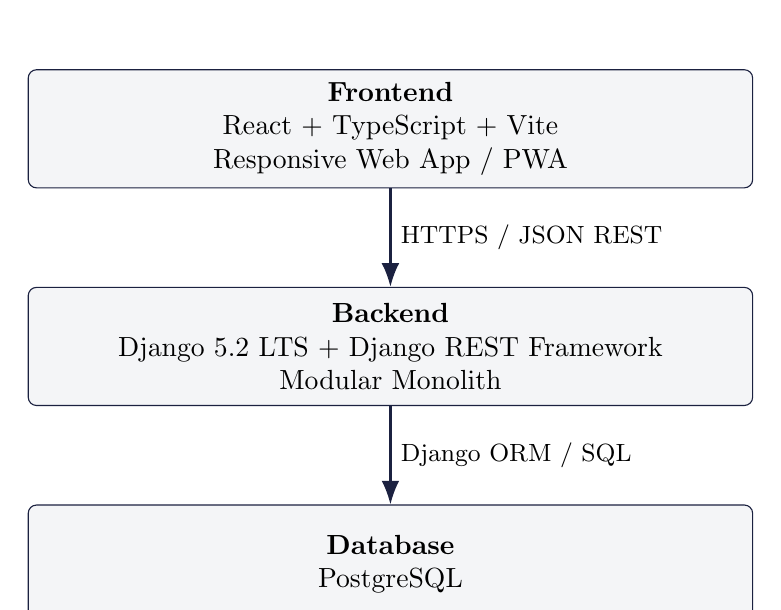
\begin{tikzpicture}[
  node distance=1.25cm,
  box/.style={draw=InkSoft, rounded corners=3pt, align=center, minimum width=9.2cm, minimum height=1.5cm, fill=CodeBg},
  arrow/.style={-{Latex[length=3mm]}, thick, draw=InkSoft}
]
\node[box] (client) {\textbf{Frontend}\\ \eng{React + TypeScript + Vite}\\ Responsive Web App / PWA};
\node[box, below=of client] (api) {\textbf{Backend}\\ \eng{Django 5.2 LTS + Django REST Framework}\\ Modular Monolith};
\node[box, below=of api] (db) {\textbf{Database}\\ \eng{PostgreSQL}};
\draw[arrow] (client) -- node[right]{\small \eng{HTTPS / JSON REST}} (api);
\draw[arrow] (api) -- node[right]{\small \eng{Django ORM / SQL}} (db);
\end{tikzpicture}
\end{center}

این ساختار برای Core MVP کافی است.

\section{نمودار فاز Realtime}

بعداً، فقط هنگام پیاده‌سازی Sync و Messaging:

\begin{center}
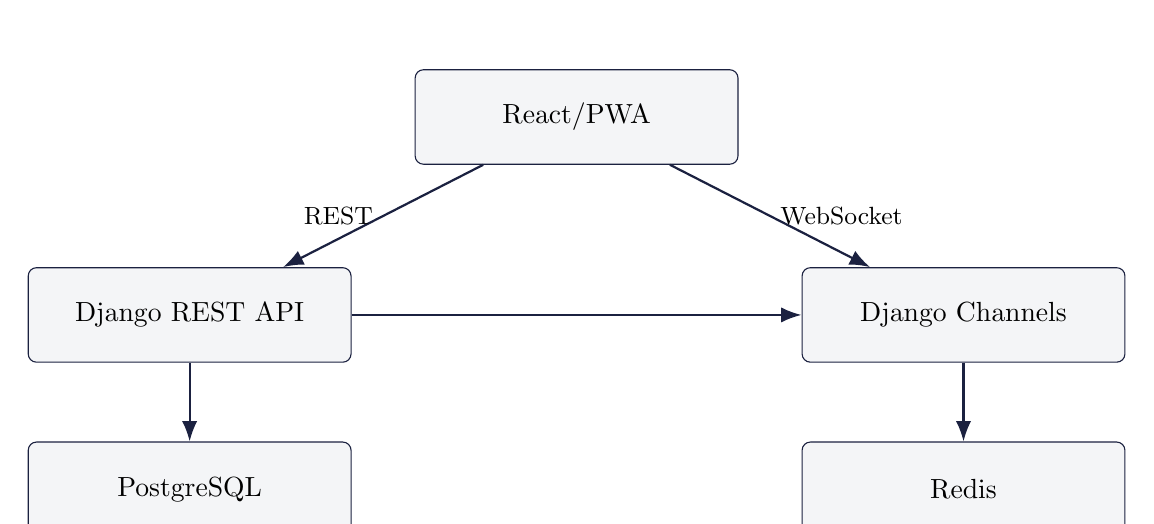
\begin{tikzpicture}[
  node distance=1.0cm and 1.3cm,
  box/.style={draw=InkSoft, rounded corners=3pt, align=center, minimum width=4.1cm, minimum height=1.2cm, fill=CodeBg},
  arrow/.style={-{Latex[length=2.6mm]}, thick, draw=InkSoft}
]
\node[box] (client) {React/PWA};
\node[box, below left=1.3cm and 0.8cm of client] (rest) {Django REST API};
\node[box, below right=1.3cm and 0.8cm of client] (ws) {Django Channels};
\node[box, below=of rest] (db) {PostgreSQL};
\node[box, below=of ws] (redis) {Redis};
\draw[arrow] (client) -- node[left]{\small REST} (rest);
\draw[arrow] (client) -- node[right]{\small WebSocket} (ws);
\draw[arrow] (rest) -- (db);
\draw[arrow] (ws) -- (redis);
\draw[arrow] (rest) -- (ws);
\end{tikzpicture}
\end{center}

\begin{warningbox}
WebSocket منبع حقیقت نیست. ابتدا تغییر باید در PostgreSQL Commit شود؛ سپس Event برای Device دیگر ارسال شود.
\end{warningbox}

\section{مرزهای Backend}

ماژول‌های پیشنهادی:

\begin{latin}
\begin{lstlisting}
backend/
  config/
  apps/
    accounts/
    content/
    creators/
    engagement/
    library/
    recommendations/
    moderation/
    messaging/       # later
    notifications/   # later
\end{lstlisting}
\end{latin}

\subsection{accounts}

مسئول:
\begin{itemize}
  \item User؛
  \item Profile settings؛
  \item UI language؛
  \item Interest selection؛
  \item Authentication-related domain data.
\end{itemize}

\subsection{content}

مسئول:
\begin{itemize}
  \item Idea؛
  \item Source؛
  \item Topic؛
  \item Publication status؛
  \item Reading time.
\end{itemize}

\subsection{creators}

مسئول:
\begin{itemize}
  \item CreatorProfile؛
  \item Follow؛
  \item public creator data.
\end{itemize}

\subsection{engagement}

مسئول:
\begin{itemize}
  \item Spark؛
  \item Save؛
  \item Comment.
\end{itemize}

\subsection{library}

مسئول:
\begin{itemize}
  \item Saved ideas view؛
  \item reading progress/statistics؛
  \item eBook/membership-facing data در فاز بعد.
\end{itemize}

\subsection{recommendations}

مسئول:
\begin{itemize}
  \item Candidate selection؛
  \item scoring؛
  \item related ideas؛
  \item recommendation explanation.
\end{itemize}

\subsection{moderation}

مسئول:
\begin{itemize}
  \item Report؛
  \item ModerationAction؛
  \item suspension/hide workflow.
\end{itemize}

\subsection{messaging و notifications}

در Baseline ساخته نمی‌شوند. فقط وقتی فاز مربوط آغاز شد.

\section{چرا Service Layer محدود استفاده می‌کنیم؟}

قرار نیست تمام Viewها فقط Wrapper روی Serviceهای پیچیده باشند. Service Layer زمانی مفید است که یک Business Operation:
\begin{itemize}
  \item چند Model را درگیر کند؛
  \item Transaction بخواهد؛
  \item از چند Endpoint فراخوانی شود؛
  \item Business Rule مستقل داشته باشد.
\end{itemize}

مثال خوب:
\begin{itemize}
  \item Recommendation scoring؛
  \item moderation action؛
  \item publish idea؛
  \item create conversation/message.
\end{itemize}

مثال نامناسب:
\begin{itemize}
  \item یک \eng{Model.objects.get()} ساده را فقط برای «تمیز به نظر رسیدن» داخل Service ببریم.
\end{itemize}

\section{اصل Dependency Direction}

ماژول‌ها باید تا حد ممکن از Domainهای پایدارتر به Domainهای سطح بالاتر وابسته باشند.

مثلاً Recommendation می‌تواند از Content و Engagement داده بگیرد؛ ولی Content نباید برای ساخت Idea به Recommendation وابسته باشد.

\section{Search}

در ابتدا Search با PostgreSQL پیاده می‌شود:
\begin{itemize}
  \item title؛
  \item body؛
  \item creator؛
  \item topic؛
  \item source.
\end{itemize}

\begin{decisionbox}
Elasticsearch/OpenSearch/Meilisearch در Baseline وجود ندارد. فقط اگر Search واقعی پروژه نشان دهد PostgreSQL ناکافی است، در آینده بررسی می‌شود.
\end{decisionbox}

\section{Media}

Cover، avatar یا فایل eBook در صورت اضافه‌شدن نباید به‌صورت Blob داخل Modelهای اصلی ذخیره شوند. Django فقط metadata/path را نگه می‌دارد و File Storage جدا مدیریت می‌شود.

در توسعه محلی می‌توان فایل‌های Media را با Storage محلی Django مدیریت کرد. CDN یا Object Storage فقط در Deployment نهایی و در صورت نیاز واقعی Scope اضافه می‌شود.

\section{اصل Graceful Degradation}

اگر Feature اختیاری مانند WebSocket، Push یا TTS در Browser قدیمی موجود نباشد:
\begin{itemize}
  \item Login باید کار کند؛
  \item Feed باید کار کند؛
  \item Read/Save/Spark/Comment باید کار کند؛
  \item Library باید کار کند.
\end{itemize}

Core Product نباید قربانی Featureهای پیشرفته شود.


\chapter{Technology Stack و دلیل انتخاب هر ابزار}

\section{Backend}

\subsection{Python 3.14.8}

نسخه موجود روی سیستم توسعه \eng{Python 3.14.8} است و با Django نصب‌شده پروژه سازگار است.

کاربرد:
\begin{itemize}
  \item زبان اصلی Backend؛
  \item Recommendation logic؛
  \item Tests؛
  \item Scripts و data utilities.
\end{itemize}

\subsection{Django 5.2.18}

Django Framework اصلی Backend است.

چیزهایی که از Django استفاده می‌کنیم:
\begin{itemize}
  \item Project configuration؛
  \item Models/ORM؛
  \item Migrations؛
  \item Authentication foundation؛
  \item Groups/Permissions؛
  \item Admin؛
  \item Middleware؛
  \item Tests؛
  \item ASGI entry point برای Realtime later.
\end{itemize}

\begin{learningbox}
Django را مثل Express با چند Library جانبی تصور نکن. Django یک Framework opinionated است و بخش زیادی از ساختار پروژه را خودش تعریف می‌کند. هدف این است که Conventionهای خود Django را یاد بگیریم، نه اینکه معماری Express را زورکی روی آن سوار کنیم.
\end{learningbox}

\subsection{Django REST Framework}

\eng{DRF} لایه API است.

کاربرد:
\begin{itemize}
  \item Serializer؛
  \item Validation؛
  \item APIView/Generic View/ViewSet؛
  \item Permission؛
  \item Pagination؛
  \item Authentication integration؛
  \item HTTP response convention.
\end{itemize}

DRF بعد از فهم Django پایه وارد پروژه می‌شود.

\subsection{PostgreSQL}

Database اصلی و production-like پروژه.

چرا:
\begin{itemize}
  \item NFR-11 صریحاً SQL relational DB می‌خواهد؛
  \item User/Idea/Topic/Save/Comment/Follow روابط واضح دارند؛
  \item Constraint و Index قوی؛
  \item Django integration عالی؛
  \item قابلیت Full Text Search و \eng{pg\_trgm} برای Search future.
\end{itemize}

\subsection{Redis - فقط بعداً}

Redis در Day 1 نصب نمی‌شود.

وقتی Realtime شروع شد:
\begin{itemize}
  \item Channels layer؛
  \item transient realtime state؛
  \item احتمالاً cache محدود.
\end{itemize}

Persistent data در Redis نگهداری نمی‌شود.

\subsection{Django Channels - فقط بعداً}

برای:
\begin{itemize}
  \item cross-device sync events؛
  \item direct messaging؛
  \item realtime notification arrival.
\end{itemize}

\subsection{Celery - فعلاً خیر}

در Baseline وجود ندارد.

فقط اگر Feature واقعی مثل:
\begin{itemize}
  \item scheduled batching؛
  \item generated TTS audio؛
  \item heavy email jobs؛
  \item long-running background processing
\end{itemize}
نیاز واقعی ایجاد کرد، دوباره ارزیابی می‌شود.

\section{Frontend}

\subsection{HTML}

قبل از React باید Semantic HTML فهمیده شود:
\begin{itemize}
  \item heading؛
  \item nav؛
  \item main؛
  \item article؛
  \item section؛
  \item form؛
  \item label/input؛
  \item button/link.
\end{itemize}

این موضوع برای Accessibility و Browser قدیمی حیاتی است.

\subsection{CSS}

موضوعات کلیدی:
\begin{itemize}
  \item Box Model؛
  \item Cascade/Specificity؛
  \item Flexbox؛
  \item Grid؛
  \item Responsive Design؛
  \item CSS Variables؛
  \item Logical Properties؛
  \item RTL/LTR؛
  \item Focus/hover/disabled states.
\end{itemize}

\subsection{JavaScript}

حتی با سابقه Node.js، Browser JavaScript Concepts باید یاد گرفته شود:
\begin{itemize}
  \item DOM؛
  \item Events؛
  \item Fetch؛
  \item Browser storage؛
  \item History/navigation؛
  \item async/await در Context شبکه.
\end{itemize}

\subsection{TypeScript}

Production Frontend با TypeScript نوشته می‌شود.

مزایا:
\begin{itemize}
  \item type safety؛
  \item refactor امن‌تر؛
  \item API data contract واضح‌تر؛
  \item autocomplete بهتر؛
  \item Skill رزومه‌ای مفید.
\end{itemize}

\subsection{React}

React برای Component-based UI استفاده می‌شود.

Conceptهای لازم:
\begin{itemize}
  \item Component؛
  \item JSX؛
  \item Props؛
  \item State؛
  \item Event handling؛
  \item Conditional rendering؛
  \item list/key؛
  \item hooks؛
  \item composition.
\end{itemize}

\subsection{Vite}

Vite Framework UI نیست. ابزار Development Server و Build است.

کاربرد:
\begin{itemize}
  \item dev server؛
  \item bundling؛
  \item environment variables frontend؛
  \item production build.
\end{itemize}

\subsection{React Router}

برای routeهایی مانند:
\begin{latin}
\begin{lstlisting}
/login
/onboarding
/feed
/ideas/:id
/explore
/library
/creators/:id
/profile
\end{lstlisting}
\end{latin}

\subsection{TanStack Query}

وقتی Frontend به API واقعی وصل شد، Server State با \eng{TanStack Query} مدیریت می‌شود:
\begin{itemize}
  \item query؛
  \item cache؛
  \item loading/error؛
  \item mutation؛
  \item invalidation؛
  \item optimistic update؛
  \item infinite pagination.
\end{itemize}

\begin{decisionbox}
Redux و Zustand از ابتدا نصب نمی‌شوند. اگر بعداً Client State واقعی و پیچیده داشتیم، آن زمان ارزیابی می‌کنیم.
\end{decisionbox}

\subsection{i18next / react-i18next}

برای ترجمه UI فارسی و انگلیسی.

\section{Testing Stack}

\subsection{Backend}

\begin{itemize}
  \item \eng{pytest}
  \item \eng{pytest-django}
\end{itemize}

\subsection{Frontend}

\begin{itemize}
  \item \eng{Vitest}
  \item \eng{React Testing Library}
\end{itemize}

\subsection{End-to-End}

\eng{Playwright} بعد از Integration واقعی Front/Back.

\subsection{Load Test}

در فاز Performance، ابزارهایی مانند \eng{Locust} برای سنجش NFRها قابل استفاده‌اند.

\section{Code Quality}

Backend:
\begin{itemize}
  \item Ruff؛
  \item type hints؛
  \item formatter/linter policy.
\end{itemize}

Frontend:
\begin{itemize}
  \item ESLint؛
  \item Prettier؛
  \item TypeScript strictness در حد عملی.
\end{itemize}

\section{ابزارهایی که انتخاب نشده‌اند}

\begin{longtable}{p{4cm}p{9cm}}
\toprule
\textbf{ابزار} & \textbf{دلیل عدم انتخاب در Baseline} \\
\midrule
Next.js & Server-side framework دوم کنار Django؛ نیاز فوری ندارد. \\
Flutter & یادگیری Dart و مسیر جدا؛ از دانش JavaScript موجود استفاده نمی‌کند. \\
Ionic/Capacitor & برای هدف Deviceهای قدیمی، محدودیت Native wrapper می‌تواند مشکل‌ساز شود؛ Web/PWA-first ساده‌تر است. \\
GraphQL & REST برای این Domain کافی و آموزشی‌تر است. \\
MongoDB & Domain رابطه‌ای است و NFR SQL می‌خواهد. \\
Elasticsearch & Search اولیه با PostgreSQL کافی است. \\
Vector DB & Embedding وجود ندارد. \\
LLM SDK & LLM در Scope نیست. \\
Microservices & Complexity غیرضروری. \\
Kubernetes & خارج از نیاز پروژه کارشناسی. \\
\bottomrule
\end{longtable}

\section{قاعده انتخاب Dependency}

قبل از \eng{pip install} یا \eng{npm install} باید بتوانیم پاسخ دهیم:
\begin{enumerate}
  \item کدام Requirement به این Package نیاز دارد؟
  \item آیا Standard Library یا Framework فعلی این کار را انجام نمی‌دهد؟
  \item این Dependency چه Complexity جدیدی می‌آورد؟
  \item چطور Test می‌شود؟
  \item اگر حذف شود چه چیزی می‌شکند؟
\end{enumerate}


\chapter{ساختار Repository و آماده‌سازی محیط}

\section{وضعیت فعلی سیستم}

مسیر فعلی Repository:
\begin{latin}
\begin{lstlisting}
/home/Pandatron/PycharmProjects/InkSight
\end{lstlisting}
\end{latin}

نام Product:
\begin{center}
\textbf{\eng{InsightInk}}
\end{center}

نسخه‌های تأییدشده:
\begin{latin}
\begin{lstlisting}
Python 3.14.8
Django 5.2.18
\end{lstlisting}
\end{latin}

Repository در حال حاضر Git دارد و \eng{.venv} نیز در Root موجود است.

\section{ساختار نهایی Monorepo}

\begin{latin}
\begin{lstlisting}
InkSight/
├── backend/
│   ├── config/
│   ├── apps/
│   ├── manage.py
│   └── ...
├── frontend/
│   ├── src/
│   ├── public/
│   ├── package.json
│   └── ...
├── docs/
│   ├── latex/
│   └── ...
├── .gitignore
├── README.md
└── ...
\end{lstlisting}
\end{latin}

Root فقط Container کل پروژه است. نه Django Project است و نه Vite Project.

\section{Virtual Environment}

\eng{.venv} در Root برای یک پروژه تک‌توسعه‌دهنده قابل قبول است.

وظیفه Virtual Environment:
\begin{itemize}
  \item جدا کردن Packageهای پروژه از Python سیستم؛
  \item reproducibility؛
  \item جلوگیری از conflict نسخه‌ها.
\end{itemize}

بررسی:
\begin{latin}
\begin{lstlisting}
.venv/bin/python --version
.venv/bin/python -m django --version
\end{lstlisting}
\end{latin}

\section{Git Cleanup قبل از کدنویسی}

وضعیت فعلی:
\begin{itemize}
  \item \filepath{.idea/} در commit اولیه Track شده؛
  \item \filepath{main.py} یک PyCharm starter است؛
  \item \filepath{.venv/} خوشبختانه Track نشده؛
  \item Branch فعلی هنگام بررسی \eng{master} بوده است.
\end{itemize}

در Phase 0 باید آگاهانه تصمیم بگیریم:
\begin{enumerate}
  \item آیا Repository را از \eng{InkSight} به \eng{InsightInk} rename کنیم؟
  \item آیا Branch را به \eng{main} تغییر دهیم؟
  \item \filepath{.idea/} را از Git خارج کنیم؟
  \item \filepath{main.py} را حذف کنیم؟
\end{enumerate}

\section{Gitignore پیشنهادی}

\begin{latin}
\begin{lstlisting}
# Python
.venv/
__pycache__/
*.py[cod]

# Secrets
.env
.env.*
!.env.example

# Django/runtime
*.sqlite3
media/
staticfiles/

# Frontend
node_modules/
dist/
coverage/

# IDE
.idea/

# OS
.DS_Store
Thumbs.db
\end{lstlisting}
\end{latin}

فقط مواردی را Ignore می‌کنیم که واقعاً Generated/Private هستند.

\section{ساخت Backend}

وقتی Phase 1 شروع شد:

\begin{latin}
\begin{lstlisting}
mkdir backend
cd backend
../.venv/bin/django-admin startproject config .
\end{lstlisting}
\end{latin}

نقطه آخر یعنی Project را داخل Current Directory بساز، نه اینکه یک Folder nested اضافی تولید شود.

خروجی تقریبی:
\begin{latin}
\begin{lstlisting}
backend/
├── config/
│   ├── __init__.py
│   ├── asgi.py
│   ├── settings.py
│   ├── urls.py
│   └── wsgi.py
└── manage.py
\end{lstlisting}
\end{latin}

\section{ساخت Frontend}

در Phase مربوط:

\begin{latin}
\begin{lstlisting}
mkdir frontend
cd frontend
npm create vite@latest . -- --template react-ts
\end{lstlisting}
\end{latin}

نسخه و Command دقیق در زمان اجرا دوباره بررسی می‌شود.

\section{PostgreSQL}

قبل از Modelهای واقعی باید:
\begin{enumerate}
  \item PostgreSQL نصب/فعال باشد؛
  \item Database پروژه ساخته شود؛
  \item User/Password محلی مشخص شود؛
  \item Django connection تست شود.
\end{enumerate}

\begin{warningbox}
برای پروژه واقعی، SQLite را به‌عنوان Database نهایی نگه نمی‌داریم. اگر برای یک تمرین آموزشی کوتاه استفاده شد، خیلی زود به PostgreSQL مهاجرت می‌کنیم.
\end{warningbox}

\section{Environment Variables}

بعداً حداقل:
\begin{latin}
\begin{lstlisting}
DJANGO_SECRET_KEY=
DJANGO_DEBUG=
DATABASE_NAME=
DATABASE_USER=
DATABASE_PASSWORD=
DATABASE_HOST=
DATABASE_PORT=
\end{lstlisting}
\end{latin}

فایل \filepath{.env} Commit نمی‌شود؛ \filepath{.env.example} بدون Secret می‌تواند Commit شود.

\section{Dependency Files}

برای Python باید یک روش reproducible انتخاب شود. گزینه‌ها:
\begin{itemize}
  \item \filepath{requirements.txt} ساده؛
  \item یا \filepath{pyproject.toml} با ابزار مدرن.
\end{itemize}

برای پروژه آموزشی، سادگی مهم است. تصمیم نهایی در Phase 0 گرفته می‌شود و بعد ثابت می‌ماند.

Frontend dependencies در \filepath{package.json} و lockfile مدیریت می‌شوند.

\section{روال روزانه توسعه}

\begin{enumerate}
  \item \tech{git status}
  \item خواندن Task همان Phase
  \item یادگیری Concept
  \item تغییر کوچک
  \item اجرای Test
  \item \tech{git diff}
  \item Update Documentation در صورت تغییر Contract
  \item Commit
\end{enumerate}

\section{Definition of Done برای Phase 0}

\begin{donebox}
Phase 0 وقتی تمام است که:
\begin{itemize}
  \item Root structure تمیز باشد؛
  \item Gitignore درست باشد؛
  \item IDE/generated files مدیریت شده باشند؛
  \item نسخه Python/Django ثبت شده باشد؛
  \item PostgreSQL آماده باشد؛
  \item Strategy dependency مشخص باشد؛
  \item اولین Commit مستندات ثبت شده باشد.
\end{itemize}
\end{donebox}


\chapter{مسیر یادگیری Python و Django}

\section{هدف این فصل}

چون Backend قبلی توسعه‌دهنده \eng{Node.js/Express} بوده، این فصل ترتیب یادگیری را طوری می‌چیند که دانش قبلی حفظ شود و تفاوت‌های Python/Django به‌صورت مرحله‌ای فهمیده شوند.

\section{Python: چیزهایی که واقعاً لازم داریم}

\subsection{مرحله P1: Syntax و Data Types}

باید بتوانی این موارد را بدون کمک توضیح بدهی و بنویسی:
\begin{itemize}
  \item variable؛
  \item \eng{str/int/float/bool/None}؛
  \item list؛
  \item tuple؛
  \item dict؛
  \item set؛
  \item if/elif/else؛
  \item for/while.
\end{itemize}

مثال:
\begin{latin}
\begin{lstlisting}[language=Python]
topics = ["science", "history", "business"]

for topic in topics:
    print(topic)
\end{lstlisting}
\end{latin}

\subsection{مرحله P2: Function}

\begin{latin}
\begin{lstlisting}[language=Python]
def calculate_reading_minutes(word_count: int) -> int:
    words_per_minute = 220
    return max(1, round(word_count / words_per_minute))
\end{lstlisting}
\end{latin}

مفاهیم:
\begin{itemize}
  \item parameter؛
  \item argument؛
  \item return؛
  \item default parameter؛
  \item type hint؛
  \item scope.
\end{itemize}

\subsection{مرحله P3: Module و Package}

در Node.js با import/export آشنا هستی. در Python نیز Code را به Moduleها تقسیم می‌کنیم.

\begin{latin}
\begin{lstlisting}[language=Python]
from recommendations.scoring import calculate_score
\end{lstlisting}
\end{latin}

باید تفاوت این‌ها را بفهمی:
\begin{itemize}
  \item file/module؛
  \item package؛
  \item import path؛
  \item \filepath{__init__.py}.
\end{itemize}

\subsection{مرحله P4: Class و Object}

Django Modelها Class هستند؛ بنابراین قبل از Model باید OOP پایه را بفهمی.

\begin{latin}
\begin{lstlisting}[language=Python]
class IdeaSummary:
    def __init__(self, title: str, score: float):
        self.title = title
        self.score = score

    def is_recommended(self) -> bool:
        return self.score >= 5
\end{lstlisting}
\end{latin}

مفاهیم:
\begin{itemize}
  \item class؛
  \item instance؛
  \item attribute؛
  \item method؛
  \item constructor؛
  \item inheritance؛
  \item composition.
\end{itemize}

\subsection{مرحله P5: Exception}

\begin{latin}
\begin{lstlisting}[language=Python]
try:
    score = calculate_score(user, idea)
except ValueError as exc:
    logger.warning("Invalid recommendation input: %s", exc)
\end{lstlisting}
\end{latin}

نباید هر Exception را با \tech{except Exception} پنهان کنیم.

\subsection{مرحله P6: Comprehension و Iterator}

در حد عملی:
\begin{latin}
\begin{lstlisting}[language=Python]
topic_ids = [topic.id for topic in idea.topics.all()]
\end{lstlisting}
\end{latin}

هدف فهم خوانایی و Lazy behavior است، نه استفاده نمایشی از Syntax پیچیده.

\section{Django از چه اجزایی تشکیل شده؟}

\subsection{Project}

\eng{Django Project} تنظیمات کل Application است.

فایل‌های اصلی:
\begin{itemize}
  \item \filepath{settings.py}
  \item \filepath{urls.py}
  \item \filepath{asgi.py}
  \item \filepath{wsgi.py}
\end{itemize}

\subsection{App}

Django App یک Domain/Capability قابل تفکیک است.

مثلاً:
\begin{latin}
\begin{lstlisting}
accounts
content
engagement
recommendations
\end{lstlisting}
\end{latin}

\begin{warningbox}
برای هر Table یک App نساز. App باید Business Responsibility داشته باشد.
\end{warningbox}

\section{URL Routing}

Express:
\begin{latin}
\begin{lstlisting}
app.get("/ideas/:id", handler)
\end{lstlisting}
\end{latin}

Django:
\begin{latin}
\begin{lstlisting}[language=Python]
path("ideas/<int:pk>/", views.idea_detail)
\end{lstlisting}
\end{latin}

DRF در مراحل بعد abstractionهای بیشتری می‌دهد، اما ابتدا باید این مسیر ساده فهمیده شود.

\section{Request و Response}

باید بفهمی:
\begin{itemize}
  \item Browser request می‌فرستد؛
  \item Django URL را Resolve می‌کند؛
  \item View اجرا می‌شود؛
  \item DB query در صورت نیاز انجام می‌شود؛
  \item Response برمی‌گردد.
\end{itemize}

\section{Model و ORM}

مثال آموزشی:
\begin{latin}
\begin{lstlisting}[language=Python]
from django.db import models

class Topic(models.Model):
    slug = models.SlugField(unique=True)
    name_fa = models.CharField(max_length=100)
    name_en = models.CharField(max_length=100)
\end{lstlisting}
\end{latin}

این Class به Table در Database نگاشت می‌شود.

باید این عملیات ORM را بلد باشی:
\begin{latin}
\begin{lstlisting}[language=Python]
Topic.objects.all()
Topic.objects.get(slug="science")
Topic.objects.filter(is_active=True)
Topic.objects.create(...)
\end{lstlisting}
\end{latin}

\section{Migration}

Migration تاریخچه تغییر Schema است.

Flow:
\begin{latin}
\begin{lstlisting}
change models.py
    ↓
python manage.py makemigrations
    ↓
inspect migration
    ↓
python manage.py migrate
\end{lstlisting}
\end{latin}

\begin{warningbox}
Migration را فایل Generated بی‌ارزش تصور نکن. بخشی از تاریخچه Schema پروژه است و باید Commit شود.
\end{warningbox}

\section{Django Admin}

Admin برای پروژه ما بسیار ارزشمند است چون قبل از ساخت Creator CMS می‌توانیم:
\begin{itemize}
  \item Topic بسازیم؛
  \item Creator ایجاد کنیم؛
  \item Source وارد کنیم؛
  \item Idea publish کنیم؛
  \item Reportها را بررسی کنیم.
\end{itemize}

بنابراین Data واقعی خیلی زود وارد Backend می‌شود.

\section{Custom User از روز اول}

\begin{warningbox}
تغییر \eng{AUTH\_USER\_MODEL} بعد از Migrationهای متعدد دردسر زیادی ایجاد می‌کند. بنابراین قبل از اولین Migration واقعی، Custom User را می‌سازیم.
\end{warningbox}

حتی اگر Custom User اولیه ساده باشد، انعطاف آینده را حفظ می‌کند.

\section{Django Authentication}

باید مفاهیم زیر را بفهمی:
\begin{itemize}
  \item password hashing؛
  \item authenticate؛
  \item login/logout؛
  \item session؛
  \item authenticated user؛
  \item group؛
  \item permission؛
  \item superuser.
\end{itemize}

\section{DRF بعد از Django پایه}

بعد از اینکه Model/View/URL را فهمیدی، می‌رویم سراغ:
\begin{itemize}
  \item Serializer؛
  \item validation؛
  \item APIView؛
  \item generic views؛
  \item ViewSet؛
  \item Router؛
  \item Permission؛
  \item Pagination.
\end{itemize}

\section{ترتیب تمرین‌های Backend}

\begin{enumerate}
  \item یک endpoint ساده health check؛
  \item Topic model + admin؛
  \item Source model؛
  \item Idea model؛
  \item query با shell؛
  \item Topic API read-only؛
  \item Idea API read-only؛
  \item create/update validation؛
  \item auth؛
  \item permissions؛
  \item engagement endpoints.
\end{enumerate}

\section{معیار فهم}

قبل از رفتن به مرحله بعد باید بتوانی پاسخ بدهی:
\begin{itemize}
  \item Model چه فرقی با Serializer دارد؟
  \item Migration دقیقاً چه چیزی را تغییر می‌دهد؟
  \item QuerySet چیست؟
  \item چرا \eng{ForeignKey} با IntegerField متفاوت است؟
  \item URLConf چه نقشی دارد؟
  \item Request چطور به View می‌رسد؟
  \item Permission کجا اعمال می‌شود؟
\end{itemize}


\chapter{طراحی Backend و ساختار Django}

\section{ساختار پیشنهادی}

\begin{latin}
\begin{lstlisting}
backend/
├── manage.py
├── config/
│   ├── settings.py
│   ├── urls.py
│   ├── asgi.py
│   └── wsgi.py
├── apps/
│   ├── accounts/
│   ├── content/
│   ├── creators/
│   ├── engagement/
│   ├── library/
│   ├── recommendations/
│   ├── moderation/
│   ├── messaging/
│   └── notifications/
└── tests/
\end{lstlisting}
\end{latin}

در عمل ممکن است Testهای هر App داخل همان App باشند. هدف این Diagram نشان دادن Domainهاست، نه اجبار به یک Layout خاص.

\section{config}

\filepath{config/} فقط Configuration پروژه است:
\begin{itemize}
  \item settings؛
  \item root URLs؛
  \item ASGI/WSGI؛
  \item environment-specific configuration later.
\end{itemize}

Business Model داخل config قرار نمی‌گیرد.

\section{accounts}

Modelهای احتمالی:
\begin{itemize}
  \item User با Avatar اختیاری و عمومی برای همهٔ حساب‌ها؛
  \item UserInterest؛
  \item UserPreference در صورت نیاز.
\end{itemize}

Serviceهای احتمالی:
\begin{itemize}
  \item update interests؛
  \item account data export/delete later.
\end{itemize}

\section{content}

هسته Domain:
\begin{itemize}
  \item Topic؛
  \item Source؛
  \item Idea؛
  \item IdeaTopic در صورت نیاز به Through Model.
\end{itemize}

قواعد:
\begin{itemize}
  \item فقط Published Idea در Feed عمومی؛
  \item Hidden content در Feed ظاهر نمی‌شود؛
  \item هر Idea باید Creator و Source مشخص داشته باشد؛
  \item Language باید مشخص باشد؛
  \item estimated reading time یا محاسبه شود یا قبل از publish ثبت شود.
\end{itemize}

\section{creators}

\begin{itemize}
  \item CreatorProfile؛
  \item CreatorFollow.
\end{itemize}

CreatorProfile با OneToOne به User وصل می‌شود.

\section{engagement}

\begin{itemize}
  \item Spark؛
  \item SavedIdea؛
  \item Comment.
\end{itemize}

Spark و Save باید Unique Constraint روی \eng{(user, idea)} داشته باشند.

\section{library}

در فاز اولیه Library می‌تواند صرفاً Query روی SavedIdea باشد.

\begin{decisionbox}
Table جدا برای LibraryEntry فقط زمانی ساخته می‌شود که Requirementی وجود داشته باشد که Save و Library Item را از هم متمایز کند.
\end{decisionbox}

بعداً:
\begin{itemize}
  \item reading stats؛
  \item eBooks؛
  \item membership entitlements.
\end{itemize}

\section{recommendations}

Recommendation Model اجباری نیست.

در ابتدا:
\begin{itemize}
  \item Query candidateها؛
  \item score در Service؛
  \item response.
\end{itemize}

اگر بعداً caching لازم شد، derived data طراحی می‌شود.

\section{moderation}

\begin{itemize}
  \item Report؛
  \item ModerationAction.
\end{itemize}

این App باید Permission boundary واضح داشته باشد.

\section{Business Logic کجا قرار بگیرد؟}

قاعده ساده:

\subsection{Model}

قواعد محلی و data invariants نزدیک خود Entity.

\subsection{Serializer}

Input/output transformation و validation API-level.

\subsection{View}

HTTP orchestration: request، permission، call business logic، response.

\subsection{Service}

Business operation چندمرحله‌ای یا قابل‌استفاده مجدد.

\subsection{Selector/Query helper}

Queryهای پیچیده read-side.

\section{Transaction}

Operationهایی که چند write وابسته دارند باید Transaction داشته باشند.

مثال future:
\begin{itemize}
  \item create moderation action + change target state؛
  \item membership activation + entitlement.
\end{itemize}

\section{Signals}

Django Signals جذاب‌اند اما باید محدود استفاده شوند.

\begin{warningbox}
Business Logic مهم را پشت Signalهای نامرئی پنهان نکن. اگر یک Action بخشی از Flow اصلی است، explicit service call معمولاً قابل‌فهم‌تر است.
\end{warningbox}

Signals برای side-effectهای محدود و کاملاً مستند مناسب‌اند.

\section{Settings}

ابتدا یک \filepath{settings.py} ساده کافی است. اگر بعداً Production/Development تفاوت زیاد شد می‌توان split کرد.

اصل:
\begin{itemize}
  \item Secret از env؛
  \item DEBUG در production false؛
  \item Database config از env؛
  \item Allowed hosts مشخص؛
  \item CORS/CSRF بر اساس deployment واقعی.
\end{itemize}

\section{Logging}

از \eng{print()} برای Debug موقت می‌توان استفاده کرد، اما Logging واقعی باید از Python logging/Django logging استفاده کند.

سطوح:
\begin{itemize}
  \item DEBUG؛
  \item INFO؛
  \item WARNING؛
  \item ERROR.
\end{itemize}

اطلاعات حساس نباید log شود.

\section{Admin strategy}

برای هر Model لازم نیست Admin بسیار پیچیده بسازیم.

ولی برای:
\begin{itemize}
  \item Idea؛
  \item Source؛
  \item Topic؛
  \item CreatorProfile؛
  \item Report
\end{itemize}
List display، search و filters مفید هستند.

\section{Seed data}

برای توسعه، Dataset کوچک و deterministic می‌سازیم:
\begin{itemize}
  \item چند User؛
  \item چند Creator؛
  \item 10-20 Topic؛
  \item چند Source از هر نوع؛
  \item حداقل 30-50 Idea برای Feed/Recommendation test.
\end{itemize}

این داده‌ها باید یا Fixture/Management Command قابل تکرار باشند، نه ورود دستی غیرقابل بازسازی.

\section{Management Command}

یک Command مثل:
\begin{latin}
\begin{lstlisting}
python manage.py seed_demo
\end{lstlisting}
\end{latin}
می‌تواند Demo data بسازد.

این بخش بعد از فهم basics اضافه می‌شود.

\section{Backend Definition of Done}

هر Backend feature:
\begin{itemize}
  \item Model/constraint درست؛
  \item Migration؛
  \item validation؛
  \item permission؛
  \item tests؛
  \item API docs؛
  \item admin/data setup در صورت لازم.
\end{itemize}


\chapter{طراحی Database و مدل داده}

\section{اصل طراحی}

NFR-11 استفاده از Relational SQL را مشخص می‌کند. Domain نیز به‌شدت Relation-oriented است؛ بنابراین PostgreSQL انتخاب طبیعی است.

\section{User}

\begin{latin}
\begin{lstlisting}
User
- id
- email
- password_hash (managed by Django)
- display_name
- preferred_ui_language
- is_active
- is_staff
- date_joined
- created_at / updated_at if needed
\end{lstlisting}
\end{latin}

\begin{decisionbox}
Custom User Model قبل از اولین Migration واقعی ساخته می‌شود.
\end{decisionbox}

\section{CreatorProfile}

\begin{latin}
\begin{lstlisting}
CreatorProfile
- id
- user_id -> User (OneToOne)
- bio_fa
- bio_en
- avatar
- is_verified
- created_at
\end{lstlisting}
\end{latin}

\section{Topic}

\begin{latin}
\begin{lstlisting}
Topic
- id
- slug
- name_fa
- name_en
- is_active
\end{lstlisting}
\end{latin}

Slug باید unique باشد.

\section{UserInterest}

\begin{latin}
\begin{lstlisting}
UserInterest
- user_id
- topic_id
- created_at
\end{lstlisting}
\end{latin}

Constraint:
\begin{latin}
\begin{lstlisting}
UNIQUE(user_id, topic_id)
\end{lstlisting}
\end{latin}

\section{Source}

Source کار اصلی است که Idea از آن آمده:

\begin{latin}
\begin{lstlisting}
Source
- id
- type: BOOK | ARTICLE | MOVIE | PODCAST
- title
- original_creator_text or structured relation if later needed
- language
- external_url (optional)
- cover (optional)
- metadata (limited)
\end{lstlisting}
\end{latin}

\begin{warningbox}
Source Creator با InsightInk Creator لزوماً یک چیز نیست. مثلاً یک کاربر InsightInk ممکن است درباره کتاب یک نویسنده خارجی Idea بنویسد.
\end{warningbox}

\section{Idea}

\begin{latin}
\begin{lstlisting}
Idea
- id
- creator_id -> CreatorProfile
- source_id -> Source
- language
- title
- body
- estimated_read_seconds
- status: DRAFT | PUBLISHED | HIDDEN
- published_at
- created_at
- updated_at
\end{lstlisting}
\end{latin}

Relation:
\[
Idea \leftrightarrow Topic
\]

\section{Spark}

\begin{latin}
\begin{lstlisting}
Spark
- user_id
- idea_id
- created_at

UNIQUE(user_id, idea_id)
\end{lstlisting}
\end{latin}

\section{SavedIdea}

\begin{latin}
\begin{lstlisting}
SavedIdea
- user_id
- idea_id
- saved_at
- last_opened_at (optional)

UNIQUE(user_id, idea_id)
\end{lstlisting}
\end{latin}

\section{Comment}

\begin{latin}
\begin{lstlisting}
Comment
- id
- author_id -> User
- idea_id -> Idea
- body
- status: VISIBLE | HIDDEN | DELETED
- created_at
- updated_at
\end{lstlisting}
\end{latin}

Nested Comment در Source requirement ضروری نیست و فعلاً اضافه نمی‌شود.

\section{CreatorFollow}

\begin{latin}
\begin{lstlisting}
CreatorFollow
- user_id
- creator_id
- created_at

UNIQUE(user_id, creator_id)
\end{lstlisting}
\end{latin}

\section{ReadingEvent}

برای Story «چند Idea این ماه خواندم» باید اول تعریف Read را مشخص کنیم.

Model احتمالی:
\begin{latin}
\begin{lstlisting}
ReadingEvent
- id
- user_id
- idea_id
- occurred_at
\end{lstlisting}
\end{latin}

\begin{warningbox}
قبل از تعریف دقیق «read»، این Table را نساز. صرف باز شدن صفحه ممکن است معادل خواندن واقعی نباشد.
\end{warningbox}

\section{Report}

\begin{latin}
\begin{lstlisting}
Report
- id
- reporter_id
- target_type
- target_id
- reason
- details
- status
- created_at
- resolved_at
\end{lstlisting}
\end{latin}

برای Generic target باید بین GenericForeignKey و Tableهای مشخص تصمیم بگیریم. برای پروژه آموزشی، سادگی و Queryability مهم‌تر از Generic abstraction است.

\section{ModerationAction}

\begin{latin}
\begin{lstlisting}
ModerationAction
- id
- moderator_id
- report_id (optional)
- action_type
- target information
- note
- created_at
\end{lstlisting}
\end{latin}

\section{Messaging - later}

\begin{latin}
\begin{lstlisting}
Conversation
- id
- created_at

ConversationParticipant
- conversation_id
- user_id

Message
- id
- conversation_id
- sender_id
- body
- created_at
- read_at
\end{lstlisting}
\end{latin}

برای Scope اولیه Conversation بین Reader و Creator است.

\section{Notification - later}

\begin{latin}
\begin{lstlisting}
Notification
- id
- recipient_id
- type
- payload
- read_at
- created_at

NotificationPreference
- user_id
- notification_type
- enabled
\end{lstlisting}
\end{latin}

\section{Membership/eBook - later}

\begin{latin}
\begin{lstlisting}
Ebook
- id
- source_id
- title
- language
- file_metadata
- access_level

Membership
- id
- user_id
- provider_reference
- status
- plan
- period_start
- period_end
\end{lstlisting}
\end{latin}

Raw card data جایی در Schema ما ندارد.

\section{ERD مفهومی}

\begin{center}
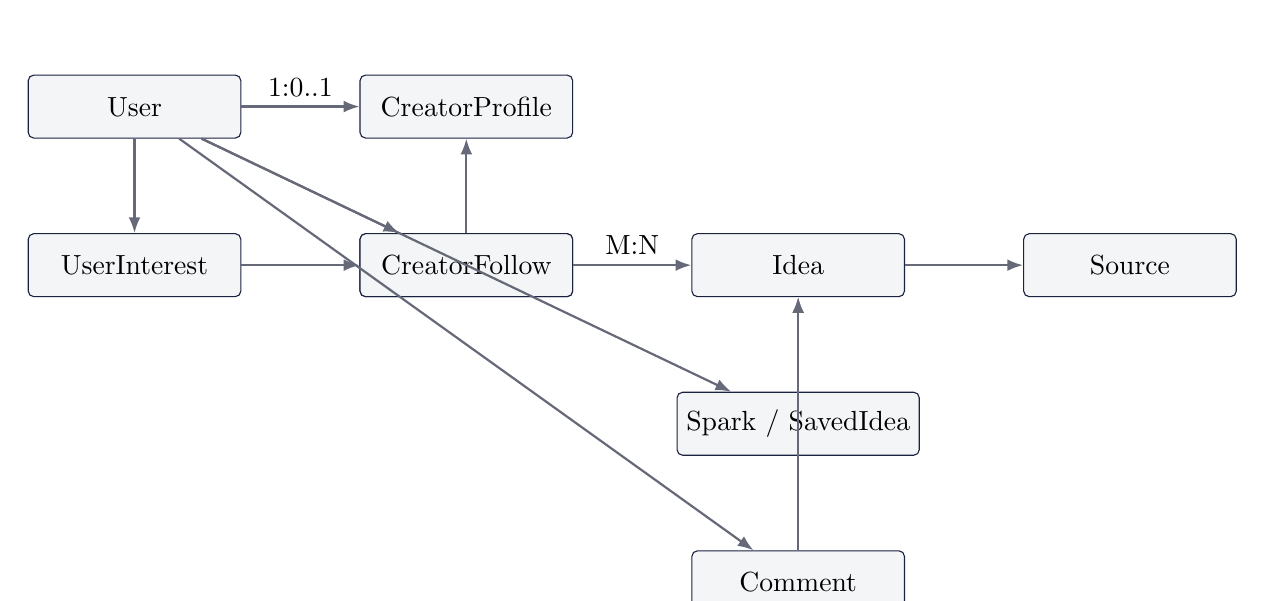
\begin{tikzpicture}[
  node distance=1.2cm and 1.5cm,
  entity/.style={draw=InkSoft, rounded corners=2pt, fill=CodeBg, minimum width=2.7cm, minimum height=0.8cm, align=center},
  rel/.style={-{Latex[length=2mm]}, draw=Ash, thick}
]
\node[entity] (user) {User};
\node[entity, right=of user] (creator) {CreatorProfile};
\node[entity, below=of user] (interest) {UserInterest};
\node[entity, right=of interest] (topic) {Topic};
\node[entity, right=of topic] (idea) {Idea};
\node[entity, right=of idea] (source) {Source};
\node[entity, below=of idea] (spark) {Spark / SavedIdea};
\node[entity, below=of creator] (follow) {CreatorFollow};
\node[entity, below=of spark] (comment) {Comment};

\draw[rel] (user) -- node[above]{1:0..1} (creator);
\draw[rel] (user) -- (interest);
\draw[rel] (interest) -- (topic);
\draw[rel] (topic) -- node[above]{M:N} (idea);
\draw[rel] (idea) -- (source);
\draw[rel] (user) -- (spark);
\draw[rel] (spark) -- (idea);
\draw[rel] (user) -- (follow);
\draw[rel] (follow) -- (creator);
\draw[rel] (user) -- (comment);
\draw[rel] (comment) -- (idea);
\end{tikzpicture}
\end{center}

\section{Index Strategy}

Index روی Fieldهایی که مرتب Filter/Sort می‌شوند:
\begin{itemize}
  \item Idea.status؛
  \item Idea.published\_at؛
  \item Idea.language؛
  \item Topic.slug؛
  \item Source.type؛
  \item Notification recipient/read state later.
\end{itemize}

Many-to-many join tableها و Foreign Keyها معمولاً Index مناسب دارند، ولی باید Query plan را بعداً بررسی کنیم.

\section{Normalization}

اصل:
\begin{itemize}
  \item داده تکراری را بی‌دلیل Duplicate نکن؛
  \item Relation واقعی را ForeignKey کن؛
  \item JSONField فقط برای metadata واقعاً flexible؛
  \item Denormalization فقط بعد از Evidence performance.
\end{itemize}

\section{Migration Rules}

\begin{enumerate}
  \item Model را تغییر بده؛
  \item \tech{makemigrations}؛
  \item فایل Migration را بخوان؛
  \item \tech{migrate}؛
  \item Test؛
  \item Commit Model + Migration با هم.
\end{enumerate}


\chapter{REST API، Authentication و Roleها}

\section{API Base}

تمام Endpointهای Versioned:
\begin{latin}
\begin{lstlisting}
/api/v1/
\end{lstlisting}
\end{latin}

فرمت اصلی:
\begin{latin}
\begin{lstlisting}
Content-Type: application/json
\end{lstlisting}
\end{latin}

\section{HTTP Methodها}

\begin{longtable}{p{2.6cm}p{10cm}}
\toprule
\textbf{Method} & \textbf{کاربرد} \\
\midrule
GET & خواندن Resource \\
POST & ساخت Resource یا Action non-idempotent \\
PUT & جایگزینی/Action idempotent در طراحی مناسب \\
PATCH & تغییر بخشی از Resource \\
DELETE & حذف Resource یا Relationship \\
\bottomrule
\end{longtable}

\section{Endpointهای Core پیشنهادی}

\subsection{Account}

\begin{latin}
\begin{lstlisting}
POST   /api/v1/auth/register/
POST   /api/v1/auth/login/
POST   /api/v1/auth/logout/

GET    /api/v1/me/
PATCH  /api/v1/me/
PUT    /api/v1/me/avatar/
DELETE /api/v1/me/avatar/

GET    /api/v1/me/interests/
PUT    /api/v1/me/interests/
\end{lstlisting}
\end{latin}

\subsection{Feed/Idea}

\begin{latin}
\begin{lstlisting}
GET    /api/v1/feed/
GET    /api/v1/ideas/{id}/
GET    /api/v1/ideas/{id}/related/
\end{lstlisting}
\end{latin}

\subsection{Engagement}

\begin{latin}
\begin{lstlisting}
PUT    /api/v1/ideas/{id}/spark/
DELETE /api/v1/ideas/{id}/spark/

PUT    /api/v1/ideas/{id}/save/
DELETE /api/v1/ideas/{id}/save/

GET    /api/v1/ideas/{id}/comments/
POST   /api/v1/ideas/{id}/comments/
DELETE /api/v1/comments/{id}/
POST   /api/v1/comments/{id}/report/
\end{lstlisting}
\end{latin}

Spark/Save باید idempotent طراحی شوند؛ یعنی تکرار PUT duplicate نسازد.

\subsection{Library}

\begin{latin}
\begin{lstlisting}
GET    /api/v1/library/saved/
GET    /api/v1/library/stats/
\end{lstlisting}
\end{latin}

\subsection{Creator}

\begin{latin}
\begin{lstlisting}
GET    /api/v1/creators/
GET    /api/v1/creators/{id}/
PUT    /api/v1/creators/{id}/follow/
DELETE /api/v1/creators/{id}/follow/
\end{lstlisting}
\end{latin}

\subsection{Search}

\begin{latin}
\begin{lstlisting}
GET    /api/v1/search/?q=...
GET    /api/v1/topics/
GET    /api/v1/topics/{slug}/ideas/
\end{lstlisting}
\end{latin}

\subsection{Recommendation}

\begin{latin}
\begin{lstlisting}
GET    /api/v1/recommendations/
GET    /api/v1/ideas/{id}/related/
\end{lstlisting}
\end{latin}

هیچ Completion/Chat endpoint وجود ندارد.

\section{Pagination}

Feed برای long-running content بهتر است Cursor-like pagination داشته باشد تا Insert شدن محتوای جدید duplicate/missing کمتری ایجاد کند.

Response مفهومی:
\begin{latin}
\begin{lstlisting}
{
  "next": "opaque-cursor",
  "previous": null,
  "results": [...]
}
\end{lstlisting}
\end{latin}

Implementation دقیق با DRF در زمان فاز Feed انتخاب می‌شود.

\section{Authentication}

Authentication پاسخ می‌دهد:
\begin{center}
«این Request متعلق به چه کسی است؟»
\end{center}

نیازها:
\begin{itemize}
  \item email/password؛
  \item secure password hash؛
  \item login/logout؛
  \item password reset؛
  \item authenticated API request؛
  \item login روی Device دیگر.
\end{itemize}

Social Login در Source آمده اما هنوز Scope نهایی آن Open Question است.

\section{Session یا Token؟}

تصمیم قفل‌شده پروژه استفاده از Django Session/Cookie authentication با
\eng{DRF SessionAuthentication} و topology ترجیحی same-origin برای Frontend و API است.
در Production، Session cookie باید Secure و HttpOnly باشد و CSRF protection فعال بماند.

هویت canonical حساب، Email اجباری و Unique است. Custom User همچنان از
\eng{AbstractUser} ارث می‌برد، فیلد Username حذف می‌شود و
\eng{USERNAME\_FIELD = "email"} خواهد بود.

\begin{warningbox}
JWT، DRF TokenAuthentication، Bearer/Refresh token سفارشی و OAuth/Social auth بدون
نیاز اثبات‌شده و تصمیم معماری جدید اضافه نمی‌شوند.
\end{warningbox}

\section{Authorization}

Authorization پاسخ می‌دهد:
\begin{center}
«این کاربر اجازه انجام این Action روی این Object را دارد؟»
\end{center}

\section{Reader}

Permissionهای اصلی:
\begin{itemize}
  \item read public content؛
  \item save/spark؛
  \item comment؛
  \item follow؛
  \item report؛
  \item own profile/interests؛
  \item message creator later.
\end{itemize}

\section{Creator}

همه قابلیت‌های Reader +:
\begin{itemize}
  \item creator profile؛
  \item own idea publishing/editing در صورت ساخت UI/API؛
  \item own statistics؛
  \item message reply.
\end{itemize}

Object ownership حیاتی است.

\section{Moderator}

\begin{itemize}
  \item view reports؛
  \item review flagged content؛
  \item hide/remove طبق policy؛
  \item resolve report؛
  \item محدودیت‌های تعریف‌شده.
\end{itemize}

نمی‌تواند:
\begin{itemize}
  \item Moderator بسازد؛
  \item Admin بسازد؛
  \item هر تنظیم سیستمی را تغییر دهد.
\end{itemize}

\section{Admin}

دسترسی کامل. در Django معمولاً با Superuser و permissionهای کامل نگاشت می‌شود.

\section{Group/Permission Strategy}

نگاشت پیشنهادی:
\begin{latin}
\begin{lstlisting}
Reader    -> authenticated user
Creator   -> User + CreatorProfile + creator permissions
Moderator -> Moderator Group (+ limited staff/admin access)
Admin     -> superuser
\end{lstlisting}
\end{latin}

\section{Object-Level Permission Example}

سناریو:
\begin{itemize}
  \item Creator A Idea A را دارد؛
  \item Creator B لاگین است.
\end{itemize}

Creator B نباید بتواند:
\begin{latin}
\begin{lstlisting}
PATCH /api/v1/ideas/A/
\end{lstlisting}
\end{latin}

حتی اگر Role او Creator باشد.

\section{Validation Error Format}

Error response باید قابل پیش‌بینی باشد. مثال مفهومی:
\begin{latin}
\begin{lstlisting}
{
  "errors": {
    "body": ["This field may not be blank."]
  }
}
\end{lstlisting}
\end{latin}

فرمت نهایی هنگام DRF setup مشخص می‌شود.

\section{OpenAPI}

بعد از شکل‌گرفتن API:
\begin{itemize}
  \item Schema OpenAPI تولید می‌شود؛
  \item Endpointها و Request/Response ثبت می‌شوند؛
  \item در صورت ارزش عملی، Typeهای Frontend از Schema تولید می‌شوند.
\end{itemize}

\section{API Definition of Done}

هر Endpoint:
\begin{itemize}
  \item method/path مشخص؛
  \item auth requirement؛
  \item permission؛
  \item validation؛
  \item success/error status؛
  \item test؛
  \item documentation.
\end{itemize}


\chapter{مسیر یادگیری Frontend از صفر}

\section{چرا مستقیم وارد React نمی‌شویم؟}

React روی مفاهیم Browser و JavaScript بنا شده است. اگر DOM، Event، Fetch و State را نفهمیم، React تبدیل به مجموعه‌ای از دستورهای حفظی می‌شود.

بنابراین یادگیری Frontend در این پروژه مرحله‌ای است.

\section{مرحله F1: HTML}

موضوعات:
\begin{itemize}
  \item document structure؛
  \item semantic elements؛
  \item heading hierarchy؛
  \item link vs button؛
  \item form؛
  \item label/input؛
  \item nav/main/article/section؛
  \item accessibility basics.
\end{itemize}

تمرین پروژه:
\begin{itemize}
  \item Idea Card استاتیک؛
  \item Login form؛
  \item Navigation ساده.
\end{itemize}

\begin{learningbox}
اول باید بفهمی چرا \eng{button} برای Action و \eng{a} برای Navigation استفاده می‌شود. این تفاوت بعداً روی Accessibility و Keyboard behavior تأثیر دارد.
\end{learningbox}

\section{مرحله F2: CSS}

موضوعات:
\begin{itemize}
  \item selector؛
  \item cascade؛
  \item specificity؛
  \item box model؛
  \item width/height؛
  \item margin/padding؛
  \item Flexbox؛
  \item Grid؛
  \item responsive؛
  \item media query؛
  \item CSS variable؛
  \item logical properties؛
  \item RTL/LTR.
\end{itemize}

تمرین:
\begin{itemize}
  \item بازسازی IdeaCard پروتوتایپ؛
  \item ساخت Bottom Navigation؛
  \item responsive کردن Feed.
\end{itemize}

\section{مرحله F3: Browser JavaScript}

با وجود تجربه Node.js، باید Browser-specific concepts را یاد بگیری.

\subsection{DOM}

\begin{latin}
\begin{lstlisting}
const button = document.querySelector("#save-button");
button.addEventListener("click", () => {
  console.log("saved");
});
\end{lstlisting}
\end{latin}

موضوعات:
\begin{itemize}
  \item DOM tree؛
  \item querySelector؛
  \item event؛
  \item event target؛
  \item form submit؛
  \item preventDefault.
\end{itemize}

\subsection{Fetch}

\begin{latin}
\begin{lstlisting}
const response = await fetch("/api/v1/ideas/");
const data = await response.json();
\end{lstlisting}
\end{latin}

باید بفهمی:
\begin{itemize}
  \item Promise؛
  \item async/await؛
  \item network failure؛
  \item HTTP error با exception جاوااسکریپت یکی نیست؛
  \item JSON parsing.
\end{itemize}

\section{مرحله F4: npm و package.json}

مفاهیم:
\begin{itemize}
  \item package؛
  \item dependency؛
  \item devDependency؛
  \item script؛
  \item lockfile؛
  \item semantic versioning در حد عملی.
\end{itemize}

\section{مرحله F5: TypeScript}

مثال JavaScript:
\begin{latin}
\begin{lstlisting}
function formatIdea(idea) {
  return idea.title;
}
\end{lstlisting}
\end{latin}

TypeScript:
\begin{latin}
\begin{lstlisting}
type Idea = {
  id: number;
  title: string;
  body: string;
};

function formatIdea(idea: Idea): string {
  return idea.title;
}
\end{lstlisting}
\end{latin}

موضوعات:
\begin{itemize}
  \item primitive types؛
  \item array/object؛
  \item type alias؛
  \item interface؛
  \item union؛
  \item optional field؛
  \item function type؛
  \item generic در حد لازم؛
  \item narrowing؛
  \item unknown vs any.
\end{itemize}

\begin{warningbox}
برای سریع شدن، \eng{any} را به Default تبدیل نکن. اگر داده API را نمی‌دانیم، Contract را تعریف می‌کنیم.
\end{warningbox}

\section{مرحله F6: React Fundamentals}

\subsection{Component}

\begin{latin}
\begin{lstlisting}
function IdeaCard() {
  return <article>...</article>;
}
\end{lstlisting}
\end{latin}

\subsection{Props}

\begin{latin}
\begin{lstlisting}
type IdeaCardProps = {
  title: string;
  readingTime: string;
};

function IdeaCard({ title, readingTime }: IdeaCardProps) {
  return (
    <article>
      <h2>{title}</h2>
      <span>{readingTime}</span>
    </article>
  );
}
\end{lstlisting}
\end{latin}

\subsection{State}

مثلاً local state برای باز/بسته بودن Menu.

\subsection{Event}

Save click، Language switch، Form submit.

\subsection{List Rendering}

Feed:
\begin{latin}
\begin{lstlisting}
{ideas.map((idea) => (
  <IdeaCard key={idea.id} idea={idea} />
))}
\end{lstlisting}
\end{latin}

\section{مرحله F7: Hooks}

به ترتیب:
\begin{itemize}
  \item \tech{useState}
  \item \tech{useEffect}
  \item \tech{useMemo} فقط وقتی دلیل وجود دارد
  \item custom hook
  \item context.
\end{itemize}

\begin{warningbox}
useEffect محل انجام هر نوع Logic نیست. قبل از استفاده باید بفهمیم آیا واقعاً Side Effect داریم یا می‌توان مقدار را مستقیم derive کرد.
\end{warningbox}

\section{مرحله F8: Routing}

Routeهای اصلی:
\begin{latin}
\begin{lstlisting}
/login
/register
/onboarding
/feed
/ideas/:ideaId
/explore
/library
/creators/:creatorId
/notifications
/profile
\end{lstlisting}
\end{latin}

Messaging later:
\begin{latin}
\begin{lstlisting}
/messages
/messages/:conversationId
\end{lstlisting}
\end{latin}

\section{مرحله F9: Server State}

بعد از اینکه fetch دستی را فهمیدی، TanStack Query وارد می‌شود.

مفاهیم:
\begin{itemize}
  \item queryKey؛
  \item queryFn؛
  \item stale/fresh؛
  \item cache؛
  \item mutation؛
  \item invalidation؛
  \item optimistic update؛
  \item infinite query.
\end{itemize}

\section{تمرین‌های Frontend در ترتیب واقعی}

\begin{enumerate}
  \item Static IdeaCard با HTML/CSS؛
  \item Responsive mobile feed؛
  \item language direction toggle؛
  \item fetch ساده از endpoint آزمایشی؛
  \item TypeScript type برای Idea؛
  \item React IdeaCard؛
  \item React feed از mock array؛
  \item Routing؛
  \item fetch real API؛
  \item TanStack Query؛
  \item Save mutation؛
  \item optimistic UI.
\end{enumerate}

\section{معیار فهم Frontend}

باید بتوانی توضیح دهی:
\begin{itemize}
  \item DOM چیست؟
  \item React چه مشکلی را نسبت به DOM manipulation دستی حل می‌کند؟
  \item Props و State چه فرقی دارند؟
  \item چرا Server State را با TanStack Query نگه می‌داریم؟
  \item TypeScript در Runtime وجود دارد یا Compile-time؟
  \item Vite چه کاری می‌کند و چه کاری نمی‌کند؟
\end{itemize}


\chapter{طراحی Frontend و تبدیل Prototype به محصول واقعی}

\section{Prototype چه چیزی به ما می‌دهد؟}

پروتوتایپ موجود 11 Screen دارد و Design Language مشخصی ارائه می‌کند:
\begin{itemize}
  \item Splash/Brand؛
  \item Interests؛
  \item Home Feed؛
  \item Idea Detail؛
  \item AI/Idea exploration concept؛
  \item Explore؛
  \item Library؛
  \item Creator Profile؛
  \item Messaging؛
  \item Notifications؛
  \item Profile/Settings.
\end{itemize}

\begin{decisionbox}
Prototype مرجع UI/UX است، نه Production code. Inline HTML/CSS/JavaScript آن به Component architecture واقعی تبدیل می‌شود.
\end{decisionbox}

\section{Design Tokenهای قابل انتقال}

Prototype رنگ‌های اصلی را مشخص کرده:
\begin{latin}
\begin{lstlisting}
--ink:        #12162B
--ink-soft:   #1B2140
--parchment:  #F5F1E6
--spark:      #F2A93B
--tide:       #3E8C8C
--ember:      #E1573A
--ash:        #9497A6
\end{lstlisting}
\end{latin}

فونت‌های Prototype:
\begin{itemize}
  \item Fraunces؛
  \item Manrope؛
  \item IBM Plex Mono.
\end{itemize}

برای UI فارسی باید خوانایی Vazirmatn یا فونت فارسی مناسب را در Product frontend ارزیابی کنیم؛ لازم نیست فونت Prototype انگلیسی برای متن فارسی استفاده شود.

\section{Theme Structure}

\begin{latin}
\begin{lstlisting}
frontend/src/theme/
├── tokens.css
├── typography.css
├── globals.css
└── components.css   # only if useful
\end{lstlisting}
\end{latin}

\section{Componentهای اصلی}

\subsection{Primitive/Shared}

\begin{itemize}
  \item Button؛
  \item IconButton؛
  \item Badge؛
  \item Avatar؛
  \item LoadingState؛
  \item ErrorState؛
  \item EmptyState.
\end{itemize}

\subsection{Domain Components}

\begin{itemize}
  \item IdeaCard؛
  \item FormatBadge؛
  \item ReadingTime؛
  \item SparkButton؛
  \item SaveButton؛
  \item CommentList؛
  \item CreatorSummary؛
  \item TopicChip؛
  \item NotificationRow؛
  \item MessageBubble later؛
  \item AudioControls later.
\end{itemize}

\section{Feature-based folders}

\begin{latin}
\begin{lstlisting}
src/
├── app/
├── api/
├── components/
├── features/
│   ├── auth/
│   ├── onboarding/
│   ├── feed/
│   ├── idea/
│   ├── explore/
│   ├── library/
│   ├── creators/
│   ├── recommendations/
│   ├── messaging/
│   ├── notifications/
│   └── profile/
├── i18n/
├── theme/
├── hooks/
└── types/
\end{lstlisting}
\end{latin}

\section{Page vs Component}

Page معمولاً:
\begin{itemize}
  \item Route-level است؛
  \item data fetching را orchestrate می‌کند؛
  \item چند Component را کنار هم می‌چیند.
\end{itemize}

Component:
\begin{itemize}
  \item بخشی از UI؛
  \item ترجیحاً مسئولیت محدود؛
  \item reusable در صورت نیاز واقعی.
\end{itemize}

\section{Feed Design}

Feed باید:
\begin{itemize}
  \item Pagination داشته باشد؛
  \item loading next page واضح باشد؛
  \item duplicate key نداشته باشد؛
  \item scroll performance قابل قبول بماند؛
  \item روی Device ضعیف Animation سنگین نداشته باشد.
\end{itemize}

در Frontend:
\begin{itemize}
  \item \eng{Infinite Query} در TanStack Query؛
  \item prefetch نزدیک انتهای لیست در صورت نیاز؛
  \item skeleton ساده، نه animation سنگین.
\end{itemize}

\section{IdeaCard Data Contract}

نمونه Type مفهومی:
\begin{latin}
\begin{lstlisting}
type IdeaCardData = {
  id: number;
  title: string;
  excerpt: string;
  language: "fa" | "en";
  source: {
    title: string;
    type: "book" | "article" | "movie" | "podcast";
  };
  creator: {
    id: number;
    displayName: string;
  };
  estimatedReadSeconds: number;
  sparkCount: number;
  commentCount: number;
  isSparked: boolean;
  isSaved: boolean;
};
\end{lstlisting}
\end{latin}

این Type باید از API Contract واقعی derive شود، نه حدس مستقل Frontend.

\section{Optimistic UI}

برای Save/Spark:
\begin{enumerate}
  \item User کلیک می‌کند؛
  \item UI فوراً state را تغییر می‌دهد؛
  \item Request ارسال می‌شود؛
  \item اگر success بود state تثبیت می‌شود؛
  \item اگر failure بود rollback + error message.
\end{enumerate}

این کار به NFR-01 کمک می‌کند.

\section{Forms}

برای Login/Register/Comment:
\begin{itemize}
  \item label واقعی؛
  \item validation message؛
  \item disabled state هنگام submit؛
  \item server error نمایش داده شود؛
  \item keyboard/mobile-friendly input؛
  \item فارسی/انگلیسی.
\end{itemize}

در ابتدا می‌توان با React state ساده Form را فهمید؛ بعد اگر Complexity بالا رفت \eng{React Hook Form} ارزیابی می‌شود. آن را از روز اول اجباری نمی‌کنیم.

\section{API Client}

یک wrapper کوچک برای:
\begin{itemize}
  \item base URL؛
  \item JSON parsing؛
  \item auth credentials/token؛
  \item common error handling.
\end{itemize}

\begin{warningbox}
یک API abstraction غول‌آسا که تمام Endpointها و State management را مخلوط کند نساز.
\end{warningbox}

\section{Responsive Strategy}

Mobile-first:
\begin{itemize}
  \item small screen baseline؛
  \item tablet enhancement؛
  \item desktop layout enhancement.
\end{itemize}

نه اینکه Desktop را بسازیم و بعد با ده‌ها media query روی موبایل جمع کنیم.

\section{Old Device UI Rules}

\begin{itemize}
  \item DOM ساده؛
  \item shadow/blur/animation محدود؛
  \item image size کنترل‌شده؛
  \item lazy load media؛
  \item avoid huge icon/UI libraries؛
  \item JS bundle کوچک؛
  \item no autoplay.
\end{itemize}

\section{Prototype Screen Mapping}

\begin{longtable}{p{4cm}p{8.5cm}}
\toprule
\textbf{Prototype Screen} & \textbf{Production Feature} \\
\midrule
Splash & onboarding intro + auth entry \\
Choose Interests & onboarding interests API + UI \\
Home Feed & paginated personalized feed \\
Idea Detail & idea/source/comments/actions \\
AI Assistant & non-LLM related/recommended ideas panel \\
Explore & search/topics/formats \\
Library & saved ideas + stats \\
Creator Profile & creator/follow/ideas \\
Message Creator & later realtime messaging \\
Notifications & later in-app notification center \\
Profile & language/interests/settings/logout \\
\bottomrule
\end{longtable}

\section{Frontend Definition of Done}

هر Screen:
\begin{itemize}
  \item responsive؛
  \item RTL/LTR؛
  \item loading؛
  \item empty؛
  \item error؛
  \item accessible name/focus؛
  \item API contract؛
  \item component test در صورت critical behavior.
\end{itemize}


\chapter{سیستم پیشنهاددهی الگوریتمی}

\section{هدف}

Recommendation باید بدون LLM بتواند:
\begin{itemize}
  \item Feed اولیه را بر اساس Interest بسازد؛
  \item با رفتار Save/Spark تطبیق پیدا کند؛
  \item Creator follow را لحاظ کند؛
  \item محتواهای مشابه را پیدا کند؛
  \item Cross-format discovery بدهد؛
  \item دلیل پیشنهاد را شفاف کند.
\end{itemize}

\section{Cold Start}

User جدید Behavior ندارد. پس Signal اول:
\[
\text{Declared Interests}
\]

مثال:
\begin{latin}
\begin{lstlisting}
User:
  Science
  Business
  History
\end{lstlisting}
\end{latin}

Ideaهای Science/Business/History Score اولیه بالاتر می‌گیرند.

\section{Signalهای اصلی}

\begin{itemize}
  \item explicit interest match؛
  \item saved-topic affinity؛
  \item sparked-topic affinity؛
  \item followed creator؛
  \item popularity؛
  \item freshness؛
  \item content-language preference؛
  \item already-seen penalty.
\end{itemize}

\section{فرمول پایه}

\[
Score(i,u) =
w_1 I +
w_2 S +
w_3 K +
w_4 F +
w_5 P +
w_6 R +
w_7 L -
w_8 V
\]

که در آن:
\begin{itemize}
  \item \(I\): Interest match؛
  \item \(S\): Save affinity؛
  \item \(K\): Spark affinity؛
  \item \(F\): Followed creator signal؛
  \item \(P\): Popularity؛
  \item \(R\): Recency/Freshness؛
  \item \(L\): Language fit؛
  \item \(V\): Viewed/consumed penalty.
\end{itemize}

وزن اولیه پیشنهادی:
\begin{longtable}{p{6.8cm}r}
\toprule
Signal & Weight فرضی \\
\midrule
Explicit interest & +5 \\
Saved topic affinity & +4 \\
Sparked topic affinity & +3 \\
Followed creator & +3 \\
Preferred content language & +2 \\
Popularity & 0 تا +1 \\
Freshness & 0 تا +1 \\
Already consumed & penalty \\
\bottomrule
\end{longtable}

\begin{warningbox}
این Weightها Requirement منبع نیستند. Hypothesis فنی هستند و باید با داده آزمایشی Tune شوند.
\end{warningbox}

\section{جلوگیری از رشد بی‌نهایت Affinity}

اگر User صدها Save روی یک Topic داشت، Score نباید خطی بی‌نهایت رشد کند.

مثال ساده:
\[
Affinity = \min(count, cap)
\]

یا Normalization به بازه مشخص.

\section{Jaccard Similarity}

برای Related Ideas:
\[
J(A,B)=\frac{|A\cap B|}{|A\cup B|}
\]

مثال:
\begin{align*}
A &= \{Productivity, Focus, Psychology\}\\
B &= \{Productivity, Focus, Habits\}\\
J(A,B) &= \frac{2}{4}=0.5
\end{align*}

مزیت:
\begin{itemize}
  \item deterministic؛
  \item قابل توضیح؛
  \item بدون Model/Embedding؛
  \item مناسب دفاع دانشگاهی.
\end{itemize}

\section{Cross-format Diversity}

اگر User Idea کتابی درباره Focus می‌بیند، Related list می‌تواند Podcast با Topic مشابه را Boost کند.

مفهوم:
\[
FinalRelatedScore = TopicSimilarity + DiversityBonus
\]

Format متفاوت نباید خودکار بهتر باشد؛ فقط Bonus کوچک برای جلوگیری از monotony.

\section{Popularity}

Popularity نباید صرفاً total sparks باشد چون محتوای قدیمی همیشه برنده می‌شود.

می‌توانیم از Normalized popularity استفاده کنیم:
\begin{itemize}
  \item sparks در بازه اخیر؛
  \item comments؛
  \item save ratio؛
  \item capped score.
\end{itemize}

برای MVP ساده نگه می‌داریم.

\section{Freshness}

Freshness می‌تواند تابعی از age باشد:
\[
Freshness = \max(0, 1 - \frac{AgeDays}{Window})
\]

مثلاً Window = 30 روز برای یک Bonus کوچک.

\section{Recommendation Explanation}

از Signal واقعی Reason می‌سازیم:
\begin{itemize}
  \item «چون Science را انتخاب کرده‌ای.»
  \item «چون چند Idea درباره Focus ذخیره کرده‌ای.»
  \item «چون این Creator را دنبال می‌کنی.»
  \item «موضوع مشابه، اما این بار از یک Podcast.»
\end{itemize}

Reason باید با Score واقعی سازگار باشد.

\section{Feed Ranking و Related Idea جدا هستند}

\subsection{Feed}

User-specific.

\subsection{Related}

Idea-specific و کمتر وابسته به User.

این دو Service جدا طراحی می‌شوند.

\section{ساختار کد پیشنهادی}

\begin{latin}
\begin{lstlisting}
apps/recommendations/
├── scoring.py
├── selectors.py
├── explanations.py
├── services.py
└── tests/
\end{lstlisting}
\end{latin}

\section{Pure Function}

مثال مفهومی:
\begin{latin}
\begin{lstlisting}[language=Python]
def weighted_score(
    interest_match: float,
    saved_affinity: float,
    sparked_affinity: float,
    followed_creator: bool,
    popularity: float,
    freshness: float,
) -> float:
    score = 0.0
    score += 5 * interest_match
    score += 4 * saved_affinity
    score += 3 * sparked_affinity
    score += 3 if followed_creator else 0
    score += popularity
    score += freshness
    return score
\end{lstlisting}
\end{latin}

در Implementation واقعی Inputها دقیق‌تر تعریف می‌شوند.

\section{Performance}

اشتباه:
\begin{latin}
\begin{lstlisting}[language=Python]
ideas = Idea.objects.all()
# calculate every idea in Python for every request
\end{lstlisting}
\end{latin}

بهتر:
\begin{enumerate}
  \item Candidateها را با DB محدود کن؛
  \item language/status/topic filter؛
  \item exclude hidden/blocked؛
  \item candidate window؛
  \item سپس Score.
\end{enumerate}

\section{Evaluation}

Testهای لازم:
\begin{itemize}
  \item cold start؛
  \item interest ranking؛
  \item save/spark adaptation؛
  \item follow boost؛
  \item language filter؛
  \item seen penalty؛
  \item cross-format diversity؛
  \item deterministic result؛
  \item latency زیر Target.
\end{itemize}

\section{TF-IDF به‌عنوان Stretch}

اگر Topic-only similarity ساده بود:
\begin{itemize}
  \item TF-IDF روی Title/Body؛
  \item Cosine Similarity؛
  \item scikit-learn.
\end{itemize}

این قابلیت Optional است و بدون آن Project کامل محسوب می‌شود.

\section{Conflict با Summarize in 30s}

Story منبع Quick Chip مثال \eng{Summarize in 30s} دارد. چون Generative AI حذف شده:
\begin{itemize}
  \item آن Story یا Deferred می‌شود؛
  \item یا به «Ideaهای کوتاه‌تر» تغییر می‌کند؛
  \item یا Short Excerpt دستی از قبل ذخیره می‌شود.
\end{itemize}

این تغییر Scope باید در گزارش نهایی صریح ذکر شود.


\chapter{Realtime Sync، Messaging و Notifications}

\section{چرا این بخش بعداً می‌آید؟}

تا وقتی Save، Library، User و Permission از طریق REST درست کار نکنند، WebSocket فقط Complexity اضافه می‌کند. بنابراین Realtime در Phase جدا وارد می‌شود.

\section{Cross-Device Sync}

نیازمندی:
\begin{itemize}
  \item Save روی Device A؛
  \item ظاهر شدن تغییر روی Device B ظرف حداکثر حدود 2 ثانیه؛
  \item نمایش pending/synced state.
\end{itemize}

\section{Flow صحیح Write}

\begin{center}
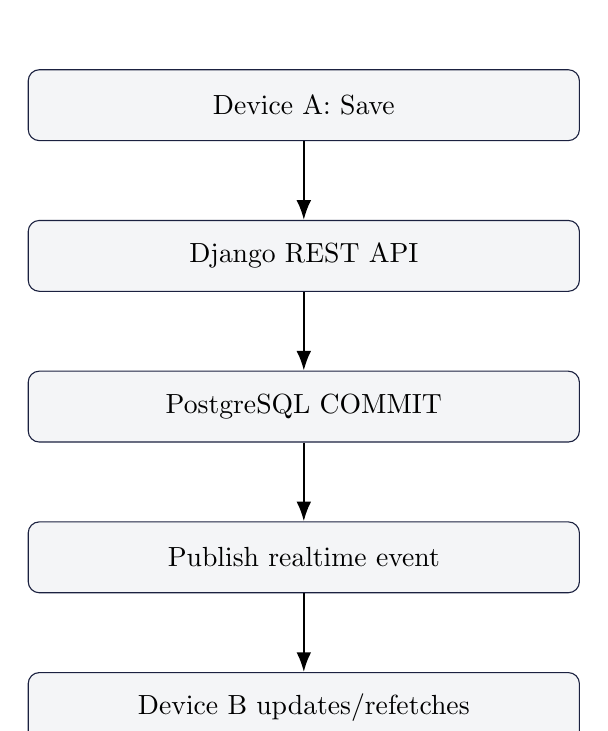
\begin{tikzpicture}[
 node distance=1cm,
 box/.style={draw=InkSoft,rounded corners,fill=CodeBg,minimum width=7cm,minimum height=0.9cm,align=center},
 arr/.style={-{Latex[length=2.5mm]},thick}
]
\node[box] (a) {Device A: Save};
\node[box,below=of a] (api) {Django REST API};
\node[box,below=of api] (db) {PostgreSQL COMMIT};
\node[box,below=of db] (evt) {Publish realtime event};
\node[box,below=of evt] (b) {Device B updates/refetches};
\draw[arr] (a)--(api);
\draw[arr] (api)--(db);
\draw[arr] (db)--(evt);
\draw[arr] (evt)--(b);
\end{tikzpicture}
\end{center}

اگر Event delivery fail شد، Save اصلی هنوز در DB موجود است.

\section{Channels و Redis}

در این فاز:
\begin{itemize}
  \item Django ASGI؛
  \item Channels Consumer؛
  \item Redis Channel Layer؛
  \item authenticated WebSocket؛
  \item reconnect handling.
\end{itemize}

\section{WebSocket Lifecycle}

Frontend باید بداند:
\begin{itemize}
  \item connecting؛
  \item connected؛
  \item disconnected؛
  \item reconnecting؛
  \item auth failure.
\end{itemize}

\section{Sync Indicator}

UI می‌تواند:
\begin{itemize}
  \item Saving...؛
  \item Saved؛
  \item Sync pending؛
  \item Sync failed / Retry
\end{itemize}
نشان دهد.

\section{Messaging Scope}

\begin{decisionbox}
Scope اولیه Messaging، Reader-to-Creator و Creator-to-Reader است؛ نه Messenger عمومی بین تمام کاربران.
\end{decisionbox}

\section{Message Flow}

\begin{enumerate}
  \item Client message submit؛
  \item authentication/participant validation؛
  \item save Message در PostgreSQL؛
  \item realtime delivery به participant online؛
  \item UI update؛
  \item history همیشه از DB قابل بازیابی.
\end{enumerate}

\section{Conversation Authorization}

هر Request برای Message باید بررسی کند:
\begin{itemize}
  \item User authenticated است؛
  \item User participant همان Conversation است؛
  \item Block policy اجازه ارسال می‌دهد؛
  \item Conversation active است.
\end{itemize}

\section{Typing Indicator}

اگر اضافه شد، Persistent data نیست و می‌تواند فقط realtime transient state باشد.

برای MVP messaging ممکن است اصلاً اضافه نشود.

\section{Read Receipt}

Story منبع الزام صریحی به read receipt ندارد. بنابراین Optional است.

\section{Block و Report}

اگر User دیگری Block شود:
\begin{itemize}
  \item ارسال پیام جدید باید محدود شود؛
  \item UI باید state را توضیح دهد؛
  \item server-side rule اجباری است.
\end{itemize}

Report conversation/message باید به moderation workflow وصل شود.

\section{Notifications}

Notification types:
\begin{itemize}
  \item creator message؛
  \item comment reply اگر later added؛
  \item new ideas from followed creators؛
  \item sync state در صورت نیاز؛
  \item moderation outcome.
\end{itemize}

\section{In-App Notification اول}

به دلیل old-device support:
\begin{decisionbox}
In-App Notification baseline است. Web Push فقط بعد از compatibility test اضافه می‌شود.
\end{decisionbox}

\section{Notification Preference}

Model server-side:
\begin{latin}
\begin{lstlisting}
NotificationPreference
- user
- type
- enabled
\end{lstlisting}
\end{latin}

بنابراین Device جدید همان preference را می‌بیند.

\section{Batching}

Source story می‌خواهد new ideas از followed creators batch شوند.

راه ساده:
\begin{itemize}
  \item eventهای مرتبط در بازه منطقی گروه شوند؛
  \item یک Notification summary ساخته شود.
\end{itemize}

اگر اجرای periodic job واقعاً لازم شد، آن زمان Task Queue بررسی می‌شود.

\section{Realtime Test}

Test دو session:
\begin{enumerate}
  \item login همان User در A و B؛
  \item save در A؛
  \item timestamp ثبت؛
  \item دریافت/update در B؛
  \item latency اندازه‌گیری؛
  \item repeat چندین بار.
\end{enumerate}

\section{Failure Scenarios}

باید تست شود:
\begin{itemize}
  \item Redis down؛
  \item WebSocket disconnect؛
  \item message duplicate attempt؛
  \item reconnect؛
  \item unauthorized conversation access؛
  \item blocked user send attempt.
\end{itemize}

\section{تعریف Done Realtime}

\begin{donebox}
Realtime وقتی Done است که REST-only correctness حفظ شده باشد، reconnect درست کار کند، unauthorized event leakage وجود نداشته باشد و Sync latency چندبار اندازه‌گیری و ثبت شده باشد.
\end{donebox}


\chapter{TTS، PWA و سازگاری با گوشی‌های قدیمی}

\section{اصل سازگاری}

بخش مهمی از کاربران فرضی ممکن است گوشی قدیمی داشته باشند. بنابراین Core experience نباید به APIهای جدید Browser وابسته باشد.

\section{Tier بندی Featureها}

\subsection{Tier 1: Core}

باید تا حد ممکن روی Browserهای قدیمی کار کند:
\begin{itemize}
  \item login؛
  \item feed؛
  \item read idea؛
  \item save؛
  \item spark؛
  \item comment؛
  \item library؛
  \item creator profile؛
  \item search.
\end{itemize}

\subsection{Tier 2: Enhancement}

ممکن است روی Device قدیمی محدود باشد:
\begin{itemize}
  \item PWA install؛
  \item Web Push؛
  \item advanced offline caching؛
  \item TTS voice features؛
  \item realtime polish.
\end{itemize}

\section{چرا Web/PWA-first؟}

Native wrapperهای مدرن ممکن است حداقل iOS/Android جدیدتری بخواهند. Web app اجازه می‌دهد Core را روی Browserهای قدیمی‌تر نیز ارزیابی کنیم.

\section{PWA چیست؟}

PWA ترکیبی از:
\begin{itemize}
  \item Web App Manifest؛
  \item Service Worker؛
  \item installability در Browserهای پشتیبانی‌شده؛
  \item caching/offline behavior محدود.
\end{itemize}

\begin{learningbox}
PWA «تبدیل خودکار سایت به اپ Native کامل» نیست. قابلیت‌ها بسته به Browser/OS فرق می‌کنند.
\end{learningbox}

\section{PWA Implementation Order}

\begin{enumerate}
  \item responsive web app کامل؛
  \item manifest؛
  \item icons؛
  \item service worker؛
  \item cache static assets؛
  \item offline fallback؛
  \item فقط بعداً cache strategy برای API.
\end{enumerate}

\begin{warningbox}
API responseهای شخصی را بدون طراحی دقیق cache نکن؛ ممکن است data stale یا privacy bug ایجاد شود.
\end{warningbox}

\section{TTS Requirement}

Source storyها می‌خواهند:
\begin{itemize}
  \item Play؛
  \item progress؛
  \item scrub؛
  \item voice selection.
\end{itemize}

\section{TTS گزینه A: Browser/Device Speech}

مزایا:
\begin{itemize}
  \item بدون server audio generation؛
  \item بدون storage cost؛
  \item بدون AI/LLM؛
  \item استفاده از Voiceهای Device.
\end{itemize}

محدودیت:
\begin{itemize}
  \item تفاوت شدید Voiceها؛
  \item Persian support وابسته به Device؛
  \item seek/scrub دقیق سخت؛
  \item behavior متفاوت در iOS/Android.
\end{itemize}

\section{TTS گزینه B: Pre-generated Audio}

مزایا:
\begin{itemize}
  \item فایل audio واقعی؛
  \item progress و scrub ساده‌تر؛
  \item behavior پایدارتر.
\end{itemize}

هزینه:
\begin{itemize}
  \item TTS provider یا engine؛
  \item storage؛
  \item background generation؛
  \item media delivery؛
  \item complexity بیشتر.
\end{itemize}

\section{تصمیم TTS}

\begin{decisionbox}
قبل از انتخاب Option A یا B، یک Prototype کوچک compatibility روی Deviceهای قدیمی ساخته می‌شود. ساده‌ترین راهی که Requirement قابل قبول را تأمین کند انتخاب می‌شود.
\end{decisionbox}

\section{Target اولیه Browser}

هنوز Guarantee رسمی نداریم.

Evaluation target:
\begin{itemize}
  \item iOS/Safari قدیمی در حدود iOS 12+ در صورت دسترسی؛
  \item Android قدیمی در حدود Android 7+؛
  \item Android فعلی؛
  \item Chrome Desktop؛
  \item Firefox Desktop.
\end{itemize}

نتیجه واقعی در Compatibility Matrix ثبت می‌شود.

\section{Frontend Performance روی Device ضعیف}

قواعد:
\begin{itemize}
  \item JS bundle کوچک؛
  \item code splitting در صورت نیاز؛
  \item تصاویر resize/compress؛
  \item lazy load image؛
  \item animation محدود؛
  \item avoid expensive blur/shadow layers؛
  \item pagination؛
  \item avoid giant DOM؛
  \item no autoplay.
\end{itemize}

\section{Legacy Build}

وقتی Dependencyهای واقعی Frontend مشخص شدند:
\begin{enumerate}
  \item Browser target واقعی تست می‌شود؛
  \item missing syntax/APIها شناسایی می‌شوند؛
  \item build target/polyfill حداقلی اضافه می‌شود.
\end{enumerate}

\begin{warningbox}
از روز اول انبوه polyfill نصب نمی‌کنیم. اول Evidence، بعد Compatibility layer.
\end{warningbox}

\section{Offline}

Offline در سطح‌های متفاوت:
\begin{itemize}
  \item static shell؛
  \item previously loaded idea؛
  \item saved ideas snapshot؛
  \item eBook download.
\end{itemize}

برای Core MVP فقط installable/offline fallback کافی است. eBook offline story later phase است.

\section{Compatibility Matrix}

\begin{longtable}{p{2.8cm}p{1.5cm}p{1.6cm}p{1.5cm}p{1.8cm}p{2.8cm}}
\toprule
Device & Core & Install & TTS & Realtime & Notes \\
\midrule
Old Android & TBD & TBD & TBD & TBD & تست واقعی \\
Old iPhone & TBD & TBD & TBD & TBD & تست واقعی \\
Current Android & TBD & TBD & TBD & TBD & \\
Chrome Desktop & TBD & N/A & TBD & TBD & \\
Firefox Desktop & TBD & N/A & TBD & TBD & \\
\bottomrule
\end{longtable}


\chapter{بین‌المللی‌سازی، RTL/LTR و Accessibility}

\section{زبان‌ها}

\begin{decisionbox}
فارسی زبان اصلی و انگلیسی زبان دوم است. هر دو از ابتدای Frontend در معماری حضور دارند.
\end{decisionbox}

\section{UI Language vs Content Language}

دو مفهوم مستقل:
\begin{itemize}
  \item \eng{preferred\_ui\_language}
  \item content language preferences.
\end{itemize}

مثال:
\begin{itemize}
  \item UI = فارسی؛
  \item content = فارسی + انگلیسی.
\end{itemize}

\section{Translation Files}

\begin{latin}
\begin{lstlisting}
src/i18n/
├── fa/
│   ├── common.json
│   ├── auth.json
│   ├── feed.json
│   └── profile.json
└── en/
    ├── common.json
    ├── auth.json
    ├── feed.json
    └── profile.json
\end{lstlisting}
\end{latin}

\section{Hard-coded text}

بعد از راه‌اندازی i18n:
\begin{latin}
\begin{lstlisting}
<button>{t("idea.save")}</button>
\end{lstlisting}
\end{latin}

بهتر از:
\begin{latin}
\begin{lstlisting}
<button>Save</button>
\end{lstlisting}
\end{latin}

\section{Direction}

در Root document:
\begin{latin}
\begin{lstlisting}
<html lang="fa" dir="rtl">
\end{lstlisting}
\end{latin}

برای English:
\begin{latin}
\begin{lstlisting}
<html lang="en" dir="ltr">
\end{lstlisting}
\end{latin}

\section{CSS Logical Properties}

ترجیح:
\begin{latin}
\begin{lstlisting}
margin-inline-start: 1rem;
padding-inline-end: 0.5rem;
text-align: start;
border-inline-start: 2px solid;
\end{lstlisting}
\end{latin}

به جای left/rightهای زیاد.

\section{Persian Text Normalization}

Search فارسی باید به تفاوت‌های:
\begin{itemize}
  \item ی/ي؛
  \item ک/ك؛
  \item نیم‌فاصله؛
  \item فاصله‌های اضافی؛
  \item punctuation
\end{itemize}
توجه کند.

\begin{warningbox}
Original content را برای Search به‌صورت destructive تغییر نده. Normalization را برای Query/indexed representation انجام بده.
\end{warningbox}

\section{Accessibility Target}

منبع WCAG 2.1 AA را می‌خواهد.

Project:
\begin{itemize}
  \item WCAG 2.1 AA minimum target؛
  \item استفاده از Improvementهای WCAG 2.2 در صورت ساده بودن؛
  \item عدم ادعای Compliance کامل بدون Audit واقعی.
\end{itemize}

\section{Semantic HTML}

قاعده:
\begin{itemize}
  \item Button واقعی برای Action؛
  \item Link واقعی برای Navigation؛
  \item Form label؛
  \item heading order؛
  \item main/nav/section/article؛
  \item table برای data table.
\end{itemize}

\section{Keyboard}

تمام Interactionهای مهم:
\begin{itemize}
  \item Tab reachable؛
  \item focus visible؛
  \item Enter/Space behavior استاندارد؛
  \item modal focus trapping اگر modal وجود دارد؛
  \item no hover-only action.
\end{itemize}

\section{Screen Reader}

Elementها باید accessible name داشته باشند.

Icon-only button:
\begin{latin}
\begin{lstlisting}
<button aria-label={t("idea.save")}>
  ...
</button>
\end{lstlisting}
\end{latin}

ARIA فقط وقتی Semantic HTML کافی نیست.

\section{Color/Contrast}

Design prototype dark theme دارد. باید Contrast واقعی:
\begin{itemize}
  \item متن اصلی؛
  \item متن secondary؛
  \item button؛
  \item focus؛
  \item error
\end{itemize}
تست شود.

\section{Touch Targets}

روی موبایل Buttonهای کوچک icon-only باید target لمس کافی داشته باشند، حتی اگر icon visual کوچک باشد.

\section{TTS مستقل از Accessibility}

TTS Feature مصرف محتواست، جای Screen Reader و Accessibility semantic را نمی‌گیرد.

\section{Testing}

\begin{itemize}
  \item keyboard manual؛
  \item browser accessibility tree؛
  \item automated axe-style checks later؛
  \item Playwright critical flows؛
  \item RTL visual inspection.
\end{itemize}

\section{Bilingual Definition of Done}

هر Screen:
\begin{itemize}
  \item fa translation؛
  \item en translation؛
  \item RTL/LTR؛
  \item long text overflow؛
  \item number/date format اگر مرتبط؛
  \item accessible labels.
\end{itemize}


\chapter{امنیت، حریم خصوصی و Moderation}

\section{اصل کلی}

Security فقط Production setting نیست؛ از Model و Permission شروع می‌شود.

\section{Password}

Django password hashing استفاده می‌شود.

ممنوع:
\begin{itemize}
  \item plaintext password؛
  \item custom crypto؛
  \item password log؛
  \item password در query string.
\end{itemize}

\section{Authentication vs Authorization}

\begin{itemize}
  \item Authentication: چه کسی؟
  \item Authorization: چه اجازه‌ای؟
\end{itemize}

هر Endpoint modifying هر دو را بررسی می‌کند.

\section{Object Ownership}

مثال‌ها:
\begin{itemize}
  \item User فقط own profile؛
  \item Creator فقط own idea؛
  \item User فقط own comment delete؛
  \item participant فقط own conversation؛
  \item Moderator طبق permission؛
  \item Admin unrestricted.
\end{itemize}

\section{CSRF}

اگر Cookie/Session auth استفاده شود، CSRF protection باید درست نگه داشته شود.

\begin{warningbox}
برای راحت شدن development، CSRF را globally disable نکن.
\end{warningbox}

\section{CORS}

CORS فقط Originهای لازم را Allow می‌کند. \eng{*} در Production برای authenticated API انتخاب مناسبی نیست.

\section{XSS}

User content مانند Comment نباید به‌عنوان raw HTML اجرا شود.

در React به‌صورت پیش‌فرض string escaping کمک می‌کند؛ از \eng{dangerouslySetInnerHTML} بدون sanitization پرهیز شود.

\section{File Upload}

اگر Avatar/Cover/eBook upload شد:
\begin{itemize}
  \item type validation؛
  \item size limit؛
  \item safe filename/storage؛
  \item authorization؛
  \item عدم اعتماد به extension.
  \item حذف فایل قبلی فقط پس از commit موفق جایگزینی.
\end{itemize}

\section{Privacy Data}

NFR-12 شامل:
\begin{itemize}
  \item reading history؛
  \item saved ideas؛
  \item personalization.
\end{itemize}

Design باید امکان:
\begin{itemize}
  \item export؛
  \item delete/anonymize؛
  \item data minimization
\end{itemize}
را بدهد.

\section{Delete Account}

قبل از Implementation باید Policy تعیین شود:
\begin{itemize}
  \item Commentها delete یا anonymize؟
  \item Creator content چه می‌شود؟
  \item Messages چطور حفظ/حذف می‌شوند؟
  \item Audit/moderation data چه می‌شود؟
\end{itemize}

این Policy باید در گزارش نهایی ثبت شود.

\section{Direct Message Privacy}

\begin{itemize}
  \item HTTPS/WSS؛
  \item participant-only access؛
  \item query filtering؛
  \item permission test؛
  \item no casual moderator browsing.
\end{itemize}

End-to-End Encryption در Scope نیست.

\section{Payment}

اگر Membership payment اجرا شد:
\begin{itemize}
  \item external provider؛
  \item no raw PAN/CVV؛
  \item provider reference؛
  \item webhook verification؛
  \item payment status state machine.
\end{itemize}

\section{Report}

Report reasonهای مشخص:
\begin{itemize}
  \item harassment؛
  \item spam؛
  \item inappropriate content؛
  \item misinformation category فقط اگر product policy مشخص شود؛
  \item other.
\end{itemize}

نباید از ابتدا سیاست‌های پیچیده و دسته‌بندی‌های زیاد بسازیم. دسته‌های نهایی Report در فاز Moderation مشخص می‌شوند.

\section{Moderation Workflow}

\begin{center}
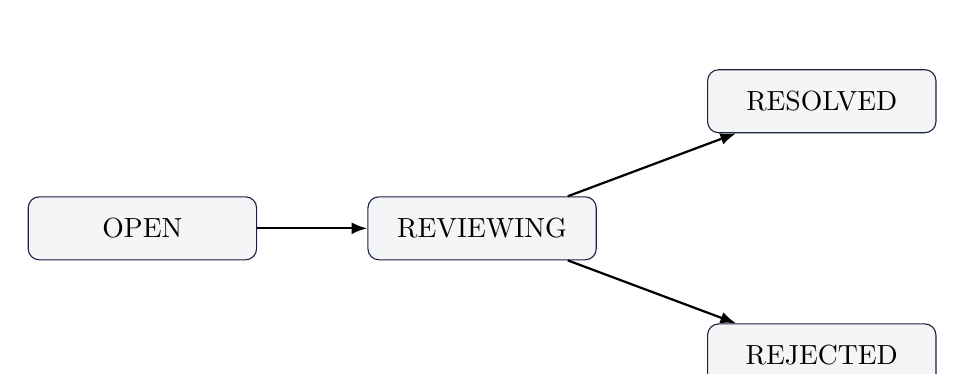
\begin{tikzpicture}[
 node distance=1.2cm and 1.4cm,
 st/.style={draw=InkSoft,rounded corners,fill=CodeBg,minimum width=2.9cm,minimum height=0.8cm,align=center},
 arr/.style={-{Latex[length=2mm]},thick}
]
\node[st] (open) {OPEN};
\node[st,right=of open] (review) {REVIEWING};
\node[st,above right=0.8cm and 1.4cm of review] (resolved) {RESOLVED};
\node[st,below right=0.8cm and 1.4cm of review] (rejected) {REJECTED};
\draw[arr] (open)--(review);
\draw[arr] (review)--(resolved);
\draw[arr] (review)--(rejected);
\end{tikzpicture}
\end{center}

\section{ModerationAction Audit}

ثبت:
\begin{itemize}
  \item actor؛
  \item target؛
  \item action type؛
  \item reason/note؛
  \item timestamp.
\end{itemize}

\section{Hidden Idea Workspace}

وضعیت فعلی Idea از \eng{Idea.status} خوانده می‌شود و
\eng{ModerationAction} فقط تاریخچه Audit است. Workspace مخصوص Moderator/Admin فقط
\eng{status=hidden} را می‌پذیرد و Draft یا Withdrawn سازنده را نمایش نمی‌دهد.
Read model آن full body، اطلاعات داخلی حساب، metadata منبع، note و تاریخچه Audit را
حذف می‌کند و تنها preview قطعی حداکثر 240 کاراکتری ارائه می‌دهد. Restore از Endpoint
اختصاصی و audited موجود انجام می‌شود.

\section{Moderator Assignment}

\begin{decisionbox}
فقط Admin حق assign/remove کردن Moderator را دارد. این Rule باید Server-side Permission test داشته باشد.
\end{decisionbox}

\section{Block}

Block باید حداقل Messaging interaction را محدود کند.

\section{Mute}

Mute می‌تواند Notification/visibility را کاهش دهد بدون Block کامل.

Semantics نهایی هنگام Feature implementation نوشته می‌شود.

\section{Rate Limiting}

Candidate:
\begin{itemize}
  \item login؛
  \item register؛
  \item comment؛
  \item report؛
  \item message؛
  \item search.
\end{itemize}

ساده‌ترین راه کافی انتخاب می‌شود.

\section{Secrets}

\filepath{.env} هرگز Commit نمی‌شود.

Secretها:
\begin{itemize}
  \item Django secret key؛
  \item DB password؛
  \item mail/payment credentials later.
\end{itemize}

\section{Logging}

Log نکن:
\begin{itemize}
  \item password؛
  \item auth token؛
  \item payment sensitive data؛
  \item private message body بی‌دلیل.
\end{itemize}

\section{Security Checklist Feature}

قبل از Done:
\begin{itemize}
  \item anonymous request test؛
  \item wrong user test؛
  \item wrong role test؛
  \item invalid data test؛
  \item ownership test؛
  \item error leakage check.
\end{itemize}


\chapter{Testing، Quality و سنجش NFRها}

\section{Test Pyramid}

\begin{center}
\begin{tikzpicture}
\draw[fill=CodeBg,draw=InkSoft] (0,0) -- (8,0) -- (6.5,1.2) -- (1.5,1.2) -- cycle;
\node at (4,0.6) {Unit Tests -- زیاد و سریع};
\draw[fill=SourceBg,draw=InkSoft] (1.5,1.2) -- (6.5,1.2) -- (5.5,2.4) -- (2.5,2.4) -- cycle;
\node at (4,1.8) {Integration/API};
\draw[fill=DecisionBg,draw=InkSoft] (2.5,2.4) -- (5.5,2.4) -- (4.7,3.6) -- (3.3,3.6) -- cycle;
\node at (4,3.0) {E2E};
\end{tikzpicture}
\end{center}

\section{Backend Unit Test}

برای:
\begin{itemize}
  \item scoring؛
  \item similarity؛
  \item helper؛
  \item validation function؛
  \item normalization.
\end{itemize}

مثال:
\begin{latin}
\begin{lstlisting}[language=Python]
def test_science_interest_ranks_science_idea_higher():
    ...
\end{lstlisting}
\end{latin}

\section{Model/DB Test}

\begin{itemize}
  \item unique save؛
  \item unique spark؛
  \item CreatorProfile one-to-one؛
  \item status constraints؛
  \item cascade/protect behavior.
\end{itemize}

\section{API Test}

سناریو:
\begin{latin}
\begin{lstlisting}
anonymous save -> 401/403
authenticated save -> success
repeat save -> no duplicate
other user deletes comment -> forbidden
moderator hides comment -> success
moderator grants moderator -> forbidden
admin grants moderator -> success
\end{lstlisting}
\end{latin}

\section{Frontend Test}

React Testing Library:
\begin{itemize}
  \item rendered text؛
  \item accessible role/name؛
  \item interaction؛
  \item loading/error؛
  \item direction.
\end{itemize}

\section{E2E}

Flow 1:
\begin{latin}
\begin{lstlisting}
register
-> choose language
-> choose interests
-> feed
\end{lstlisting}
\end{latin}

Flow 2:
\begin{latin}
\begin{lstlisting}
login
-> open idea
-> spark
-> save
-> comment
-> library
\end{lstlisting}
\end{latin}

Flow 3:
\begin{latin}
\begin{lstlisting}
creator page
-> follow
-> verify state
\end{lstlisting}
\end{latin}

Flow 4:
\begin{latin}
\begin{lstlisting}
normal user cannot moderate
moderator can review
moderator cannot assign moderator
admin can assign moderator
\end{lstlisting}
\end{latin}

\section{NFR-01}

UI perceived response زیر 100ms:
\begin{itemize}
  \item local state update؛
  \item optimistic Save/Spark؛
  \item avoid blocking main thread.
\end{itemize}

API latency جدا اندازه‌گیری می‌شود.

\section{NFR-02}

Next page Feed زیر 300ms تحت test condition تعریف‌شده.

اندازه‌گیری:
\begin{itemize}
  \item server response time؛
  \item payload size؛
  \item network condition؛
  \item render time.
\end{itemize}

\section{NFR-03}

Source «هزاران concurrent user» می‌خواهد.

برای پروژه دانشگاهی:
\begin{itemize}
  \item load test progressive؛
  \item 50، 100، 500، ...؛
  \item bottleneck report؛
  \item ادعای فقط همان چیزی که تست شده.
\end{itemize}

\section{NFR-04}

Horizontal scaling Design path مستند می‌شود. لازم نیست Kubernetes بسازیم.

\section{NFR-05}

Sync latency:
\[
t_{receive}-t_{commit} \le 2s
\]

چندین run و percentile بهتر از یک run موفق است.

\section{NFR-06}

99.9\% uptime در Project student قابل اثبات سالانه نیست.

در گزارش:
\begin{itemize}
  \item design target؛
  \item deployment assumption؛
  \item measured availability اگر test period داشتیم.
\end{itemize}

\section{NFR-07}

Idle resource:
\begin{itemize}
  \item browser devtools؛
  \item system monitor؛
  \item no polling بی‌دلیل؛
  \item no background animation.
\end{itemize}

\section{NFR-08}

اگر CDN در Deployment واقعی اجرا شد Test می‌شود؛ در غیر این صورت limitation صریح ثبت می‌شود.

\section{NFR-16}

Accessibility:
\begin{itemize}
  \item keyboard؛
  \item screen-reader spot checks؛
  \item automated audit؛
  \item contrast.
\end{itemize}

\section{NFR-17}

Recommendation latency زیر 2s. چون LLM نداریم، باید بسیار کمتر هم قابل دستیابی باشد.

\section{Test Data}

Deterministic seed:
\begin{itemize}
  \item User؛
  \item Creator؛
  \item Topic؛
  \item Source؛
  \item Idea؛
  \item Save/Spark/Follow؛
  \item Report.
\end{itemize}

\section{CI}

وقتی Test واقعی داریم:
\begin{itemize}
  \item backend test؛
  \item frontend test؛
  \item lint؛
  \item frontend build.
\end{itemize}

CI قبل از وجود Test meaningful ارزش زیادی ندارد.

\section{Coverage}

Coverage کمک‌کننده است، نه Goal.

یک Permission مهم با 100\% coverage سطحی ممکن است هنوز Bug داشته باشد. Business scenario مهم‌تر است.

\section{Quality Gate}

قبل از Merge/Commit milestone:
\begin{itemize}
  \item tests green؛
  \item lint reasonable؛
  \item no secrets؛
  \item migrations reviewed؛
  \item docs updated؛
  \item manual smoke test.
\end{itemize}


\chapter{Git Workflow، Branching و نظم توسعه}

\section{هدف}

Git فقط Backup نیست؛ تاریخچه تصمیم‌های پروژه است. برای پروژه یک‌نفره نیز باید قابل مرور باشد.

\section{Phase 0 Cleanup}

قبل از Code اصلی:
\begin{enumerate}
  \item \tech{git status}؛
  \item بررسی فایل‌های Track شده؛
  \item اضافه‌کردن \filepath{.gitignore}؛
  \item untrack کردن \filepath{.idea/} در صورت تصمیم نهایی؛
  \item حذف \filepath{main.py} starter در صورت تأیید؛
  \item تصمیم Branch \eng{master/main}؛
  \item Commit documentation.
\end{enumerate}

\section{Branch Strategy}

برای یک developer، workflow پیچیده GitFlow لازم نیست.

گزینه ساده:
\begin{itemize}
  \item \eng{main} یا \eng{master} = stable branch؛
  \item feature branch برای کارهای چندمرحله‌ای در صورت نیاز.
\end{itemize}

مثال:
\begin{latin}
\begin{lstlisting}
feature/content-models
feature/feed-api
feature/react-feed
feature/recommendation
\end{lstlisting}
\end{latin}

\section{Commit Message}

Format پیشنهادی:
\begin{latin}
\begin{lstlisting}
type(scope): short description
\end{lstlisting}
\end{latin}

Type:
\begin{itemize}
  \item feat؛
  \item fix؛
  \item test؛
  \item docs؛
  \item refactor؛
  \item chore.
\end{itemize}

مثال:
\begin{latin}
\begin{lstlisting}
feat(content): add Topic, Source and Idea models
feat(auth): add custom user model
test(engagement): prevent duplicate saves
docs(roadmap): document realtime phase
fix(i18n): correct RTL spacing in profile screen
\end{lstlisting}
\end{latin}

\section{قبل از Commit}

\begin{enumerate}
  \item \tech{git status}
  \item \tech{git diff}
  \item tests
  \item check no secret
  \item check migration
  \item documentation if contract changed
\end{enumerate}

\section{Commitهای بد}

\begin{latin}
\begin{lstlisting}
update
stuff
fix
final
final2
changes
\end{lstlisting}
\end{latin}

این پیام‌ها بعداً هیچ Contextی نمی‌دهند.

\section{Migration و Commit}

Model change و Migration مربوط باید در همان Commit باشند مگر دلیل واضح دیگری وجود داشته باشد.

\section{Lockfile}

Frontend lockfile باید Commit شود تا dependency resolution reproducible باشد.

Python dependency strategy نیز باید reproducible باشد.

\section{Secrets Check}

قبل از Push:
\begin{itemize}
  \item \filepath{.env} نباشد؛
  \item secret key نباشد؛
  \item DB password نباشد؛
  \item payment/email credential later نباشد.
\end{itemize}

\section{Tagهای Milestone}

در پایان milestoneهای مهم:
\begin{latin}
\begin{lstlisting}
v0.1-core-backend
v0.2-core-feed
v0.3-engagement
v0.4-recommendation
v1.0-bachelor-release
\end{lstlisting}
\end{latin}

Tag naming نهایی می‌تواند ساده‌تر باشد.

\section{Project Journal}

یک فایل مثل:
\begin{latin}
\begin{lstlisting}
docs/devlog/
  2026-xx-xx-phase-01.md
\end{lstlisting}
\end{latin}
اختیاری اما مفید است.

محتوا:
\begin{itemize}
  \item learned؛
  \item changed؛
  \item bug؛
  \item decision؛
  \item next.
\end{itemize}

\section{Recovery Mindset}

قبل از Command خطرناک Git:
\begin{itemize}
  \item وضعیت را بخوان؛
  \item بفهم Command چه می‌کند؛
  \item از reset --hard بدون نیاز استفاده نکن؛
  \item uncommitted work را بی‌دلیل حذف نکن.
\end{itemize}


\chapter{Roadmap اجرایی کامل پروژه}

\section{قاعده Roadmap}

هر فاز:
\[
Learn \rightarrow Build \rightarrow Test \rightarrow Document \rightarrow Commit
\]

نباید به‌خاطر جذاب بودن یک فناوری، Dependency order شکسته شود.

\section{Phase 0: Repository Foundation}

\subsection*{یادگیری}
\begin{itemize}
  \item Git status/diff/add/commit؛
  \item virtual environment؛
  \item dependency؛
  \item monorepo concept؛
  \item env variable.
\end{itemize}

\subsection*{ساخت}
\begin{itemize}
  \item repo cleanup؛
  \item .gitignore؛
  \item backend/frontend directories؛
  \item PostgreSQL ready؛
  \item dependency strategy؛
  \item documentation commit.
\end{itemize}

\begin{donebox}
Environment قابل بازسازی است و Root structure تمیز است.
\end{donebox}

\section{Phase 1: Django Foundation}

\subsection*{یادگیری}
Project/App/Settings/URL/View/Model/Migration/ORM/Admin.

\subsection*{ساخت}
\begin{itemize}
  \item Django project در backend؛
  \item PostgreSQL config؛
  \item custom User؛
  \item health endpoint؛
  \item admin superuser.
\end{itemize}

\begin{donebox}
Django با PostgreSQL اجرا می‌شود و اولین Migration با Custom User ثبت شده است.
\end{donebox}

\section{Phase 2: Core Content Models}

\subsection*{یادگیری}
ForeignKey، OneToOne، ManyToMany، constraint، index.

\subsection*{ساخت}
\begin{itemize}
  \item CreatorProfile؛
  \item Topic؛
  \item UserInterest؛
  \item Source؛
  \item Idea؛
  \item Admin config؛
  \item demo data.
\end{itemize}

\section{Phase 3: REST API Foundation}

\subsection*{یادگیری}
Serializer، validation، APIView/generic/ViewSet، HTTP status، pagination.

\subsection*{ساخت}
\begin{itemize}
  \item Topic API؛
  \item Idea API؛
  \item Creator read API؛
  \item feed baseline؛
  \item tests.
\end{itemize}

\section{Phase 4: Authentication and Roles}

\subsection*{یادگیری}
Auth vs authorization، group/permission، object ownership.

\subsection*{ساخت}
\begin{itemize}
  \item register/login/logout؛
  \item profile؛
  \item Creator permission؛
  \item Moderator group؛
  \item Admin-only moderator assignment؛
  \item tests.
\end{itemize}

\section{Phase 5: Frontend Fundamentals}

\subsection*{یادگیری}
HTML، CSS، Browser JS، npm، TypeScript، Vite.

\subsection*{ساخت}
\begin{itemize}
  \item React-TS scaffold؛
  \item theme tokens؛
  \item static mobile layout؛
  \item RTL/LTR foundation.
\end{itemize}

\section{Phase 6: React Foundation}

\subsection*{یادگیری}
Component، props، state، hooks، routing.

\subsection*{ساخت}
\begin{itemize}
  \item routing؛
  \item IdeaCard؛
  \item common states؛
  \item API client skeleton؛
  \item language switch.
\end{itemize}

\section{Phase 7: Onboarding}

\begin{itemize}
  \item intro؛
  \item register/login integration؛
  \item language selection؛
  \item interest selection؛
  \item persist interests؛
  \item first feed redirect.
\end{itemize}

\section{Phase 8: Core Feed}

\begin{itemize}
  \item paginated endpoint؛
  \item infinite query؛
  \item IdeaCard real data؛
  \item Idea Detail؛
  \item Source display؛
  \item reading estimate.
\end{itemize}

\section{Phase 9: Engagement}

\begin{itemize}
  \item Spark API/UI؛
  \item Save API/UI؛
  \item optimistic update؛
  \item Comment؛
  \item report comment؛
  \item external share.
\end{itemize}

\section{Phase 10: Personal Library}

\begin{itemize}
  \item Saved Ideas؛
  \item filters؛
  \item reading statistics فقط بعد از تعریف read؛
  \item cross-device foundation data.
\end{itemize}

\section{Phase 11: Creator Network}

\begin{itemize}
  \item Creator Profile؛
  \item Creator ideas؛
  \item Follow؛
  \item follower/spark/idea counts.
\end{itemize}

\section{Phase 12: Explore and Search}

\begin{itemize}
  \item query search؛
  \item topics؛
  \item format filters؛
  \item Persian normalization؛
  \item trending definition ساده.
\end{itemize}

\section{Phase 13: Recommendation Algorithm}

\begin{itemize}
  \item cold start؛
  \item interest score؛
  \item save/spark affinity؛
  \item follow signal؛
  \item freshness/popularity؛
  \item language fit؛
  \item Jaccard related ideas؛
  \item explanation؛
  \item evaluation.
\end{itemize}

\section{Phase 14: Realtime Sync}

در اینجا برای اولین بار:
\begin{itemize}
  \item Redis؛
  \item Channels؛
  \item WebSocket؛
  \item reconnect؛
  \item sync indicator.
\end{itemize}

\section{Phase 15: Messaging}

\begin{itemize}
  \item Conversation/Participant/Message؛
  \item reader-creator rules؛
  \item persisted history؛
  \item realtime delivery؛
  \item block/report.
\end{itemize}

\section{Phase 16: Notifications}

\begin{itemize}
  \item in-app center؛
  \item preferences؛
  \item batching؛
  \item push feasibility later.
\end{itemize}

\section{Phase 17: TTS}

\begin{enumerate}
  \item compatibility prototype؛
  \item compare browser vs generated audio؛
  \item choose simplest acceptable؛
  \item implement controls؛
  \item test Persian/English.
\end{enumerate}

\section{Phase 18: Membership/eBooks}

\begin{itemize}
  \item eBook metadata؛
  \item membership state؛
  \item entitlement؛
  \item payment only if final scope requires؛
  \item offline sample/feature if feasible.
\end{itemize}

\section{Phase 19: Moderation Completion}

\begin{itemize}
  \item report queue؛
  \item moderation action؛
  \item audit؛
  \item user restrictions؛
  \item Admin moderator management.
\end{itemize}

\section{Phase 20: Hardening}

\begin{itemize}
  \item accessibility؛
  \item old-device test؛
  \item performance؛
  \item security review؛
  \item indexes؛
  \item bilingual polish.
\end{itemize}

\section{Phase 21: Deployment}

\begin{itemize}
  \item production settings؛
  \item env؛
  \item PostgreSQL؛
  \item HTTPS؛
  \item static/media؛
  \item logs/backup.
\end{itemize}

\section{Phase 22: Final Academic Package}

\begin{itemize}
  \item final architecture diagrams؛
  \item ERD؛
  \item screenshots؛
  \item test evidence؛
  \item NFR evaluation؛
  \item limitations؛
  \item installation guide؛
  \item final report/presentation.
\end{itemize}

\section{Dependency Rules}

\begin{warningbox}
نمونه Jumpهای ممنوع:
\begin{itemize}
  \item WebSocket قبل از Save REST؛
  \item Recommendation قبل از Topic/Idea data؛
  \item Payment قبل از Library؛
  \item PWA caching پیچیده قبل از responsive app؛
  \item Redux قبل از مشاهده مشکل state management.
\end{itemize}
\end{warningbox}


\chapter{Playbookهای پیاده‌سازی Feature}

این فصل می‌گوید وقتی AI در دسترس نیست و می‌خواهی Feature جدید بسازی، چه ترتیب ثابتی را طی کنی.

\section{Playbook ساخت Model جدید}

فرض: می‌خواهی Model جدید بسازی.

\begin{enumerate}
  \item Requirement را بنویس.
  \item Entity و Relation را روی کاغذ مشخص کن.
  \item آیا Model جدید واقعاً لازم است؟
  \item Fieldها و data typeها را تعیین کن.
  \item unique/check/index را مشخص کن.
  \item deletion behavior ForeignKey را تعیین کن.
  \item Model code بنویس.
  \item \tech{makemigrations}.
  \item Migration را بخوان.
  \item \tech{migrate}.
  \item Django shell query.
  \item Model test.
  \item Admin در صورت نیاز.
  \item Commit.
\end{enumerate}

\section{Playbook ساخت API جدید}

\begin{enumerate}
  \item Use case را دقیق بنویس.
  \item Method/path را تعیین کن.
  \item Request body/query params.
  \item Authentication.
  \item Permission/object ownership.
  \item Serializer/validation.
  \item Query/Service.
  \item Response schema.
  \item status codes.
  \item happy-path test.
  \item invalid-data test.
  \item unauthorized test.
  \item object-ownership test.
  \item document.
\end{enumerate}

\section{Playbook ساخت React Screen}

\begin{enumerate}
  \item Route؛
  \item data requirement؛
  \item loading state؛
  \item empty state؛
  \item error state؛
  \item static semantic markup؛
  \item responsive CSS؛
  \item RTL/LTR؛
  \item component split؛
  \item API integration؛
  \item interaction؛
  \item accessibility؛
  \item tests.
\end{enumerate}

\section{Playbook Mutation مثل Save}

\begin{enumerate}
  \item server endpoint را اول درست کن؛
  \item idempotency؛
  \item auth/permission؛
  \item DB constraint؛
  \item API test؛
  \item frontend button؛
  \item mutation؛
  \item optimistic state؛
  \item rollback؛
  \item query invalidation/reconciliation؛
  \item cross-device event later.
\end{enumerate}

\section{Playbook Pagination}

\begin{enumerate}
  \item stable ordering؛
  \item pagination method؛
  \item page size؛
  \item endpoint tests؛
  \item frontend next page؛
  \item duplicate prevention؛
  \item loading indicator؛
  \item no-more-results state؛
  \item performance measurement.
\end{enumerate}

\section{Playbook Permission}

برای هر Action جدول بساز:

\begin{longtable}{p{5cm}cccc}
\toprule
Action & Reader & Creator & Moderator & Admin \\
\midrule
Read public idea & بله & بله & بله & بله \\
Edit own creator idea & -- & بله & policy & بله \\
Hide reported comment & -- & -- & بله & بله \\
Assign moderator & -- & -- & -- & بله \\
\bottomrule
\end{longtable}

سپس Test همان جدول را بنویس.

\section{Playbook Recommendation تغییر Weight}

\begin{enumerate}
  \item Hypothesis؛
  \item fixture scenario؛
  \item old ranking؛
  \item weight change؛
  \item unit tests؛
  \item diversity check؛
  \item latency check؛
  \item document reason.
\end{enumerate}

\section{Playbook Bug}

\begin{enumerate}
  \item reproduce؛
  \item minimal case؛
  \item log/inspect؛
  \item locate layer؛
  \item write failing test اگر ممکن؛
  \item fix؛
  \item rerun related tests؛
  \item regression check؛
  \item commit with explanation.
\end{enumerate}

\section{Playbook Database Performance}

\begin{enumerate}
  \item reproduce slow endpoint؛
  \item measure؛
  \item count queries؛
  \item inspect N+1؛
  \item \tech{select\_related/prefetch\_related}؛
  \item inspect index/query plan؛
  \item remeasure.
\end{enumerate}

Cache آخرین پاسخ پیش‌فرض نیست.

\section{Playbook Dependency}

قبل از نصب Package:
\begin{enumerate}
  \item Requirement؛
  \item alternatives؛
  \item maintenance؛
  \item size/compatibility؛
  \item security؛
  \item install؛
  \item minimal example؛
  \item integrate؛
  \item document.
\end{enumerate}

\section{Playbook Refactor}

Refactor یعنی Behavior را حفظ کن:
\begin{enumerate}
  \item tests green before؛
  \item small change؛
  \item no feature addition mixed؛
  \item tests green after؛
  \item diff review.
\end{enumerate}

\section{Playbook وقتی گیر کردی}

بدون AI:
\begin{enumerate}
  \item error را کامل بخوان؛
  \item traceback از آخر به اول؛
  \item کوچک‌ترین failing component؛
  \item official docs؛
  \item inspect input/output؛
  \item reproduce in shell/test؛
  \item تغییر یک چیز در هر بار.
\end{enumerate}

\begin{warningbox}
ده Package نصب نکن تا Bug «شاید» حل شود. اول علت را پیدا کن.
\end{warningbox}


\chapter{Deployment و Production Readiness}

\section{هدف}

Deployment این پروژه باید ساده و قابل دفاع باشد، نه نمایش DevOps.

\section{Componentهای Production}

حداقل:
\begin{itemize}
  \item Frontend static build؛
  \item Django API؛
  \item PostgreSQL؛
  \item HTTPS؛
  \item media/static handling.
\end{itemize}

بعداً اگر Realtime:
\begin{itemize}
  \item ASGI server؛
  \item Redis.
\end{itemize}

\section{Frontend Build}

\begin{latin}
\begin{lstlisting}
npm run build
\end{lstlisting}
\end{latin}

خروجی Static asset باید روی Host/CDN مناسب سرو شود.

\section{Django Production Settings}

\begin{itemize}
  \item DEBUG=False؛
  \item SECRET\_KEY از env؛
  \item ALLOWED\_HOSTS؛
  \item secure cookies؛
  \item HTTPS settings؛
  \item DB production config؛
  \item static/media config؛
  \item CORS/CSRF origin.
\end{itemize}

\section{WSGI vs ASGI}

بدون realtime، Django می‌تواند با WSGI/ASGI مناسب اجرا شود.

با Channels/WebSocket، ASGI لازم است.

باید تفاوت را هنگام فاز Realtime یاد بگیری.

\section{Static و Media}

\begin{itemize}
  \item Static = CSS/JS/build assets؛
  \item Media = user/content uploaded files.
\end{itemize}

این دو را مخلوط نکن.

\section{Database Migration Deployment}

Flow:
\begin{enumerate}
  \item backup؛
  \item deploy code؛
  \item migrate؛
  \item smoke test.
\end{enumerate}

Migration destructive باید قبل از production بررسی شود.

\section{Backup}

حداقل:
\begin{itemize}
  \item PostgreSQL dump strategy؛
  \item media backup اگر مهم؛
  \item restore test در صورت امکان.
\end{itemize}

Backup بدون تست Restore اطمینان کامل نمی‌دهد.

\section{Logging}

Production log:
\begin{itemize}
  \item request/server error؛
  \item warning؛
  \item moderation/audit where needed.
\end{itemize}

Sensitive content کمینه.

\section{Monitoring}

برای پروژه دانشگاهی:
\begin{itemize}
  \item application logs؛
  \item basic uptime observation؛
  \item database health؛
  \item error tracking اگر سرویس ساده در دسترس بود.
\end{itemize}

نباید monitoring stack سنگین بسازیم.

\section{CDN}

NFR-08 CDN می‌خواهد.

اگر Deployment واقعی امکان CDN داشت:
\begin{itemize}
  \item static/media CDN؛
  \item cache headers؛
  \item asset versioning.
\end{itemize}

اگر نداشت:
\begin{warningbox}
در گزارش نهایی صریحاً بنویس NFR-08 به‌طور کامل در محیط دانشگاهی Realize نشده است؛ به‌جای ادعای ساختگی.
\end{warningbox}

\section{Scaling Path}

اگر روزی Load زیاد شد:
\begin{itemize}
  \item چند Django instance؛
  \item reverse proxy/load balancer؛
  \item DB tuning؛
  \item cache؛
  \item Redis؛
  \item background jobs.
\end{itemize}

این‌ها Future path هستند.

\section{Release Checklist}

\begin{itemize}
  \item tests pass؛
  \item migrations applied؛
  \item DEBUG off؛
  \item secrets absent from repo؛
  \item HTTPS؛
  \item admin access secured؛
  \item sample accounts removed؛
  \item static/media reachable؛
  \item bilingual smoke test؛
  \item backup taken؛
  \item critical flow E2E.
\end{itemize}


\chapter{ردیابی کامل نیازمندی‌های منبع}

\section{هدف}

این فصل برای این است که در پایان پروژه بتوانیم نشان دهیم هر Story و NFR از کجا آمده، چگونه تفسیر شده و آیا پیاده‌سازی شده، ساده شده یا Deferred است.

\section{Epic: AI-Powered Idea Discovery}

\begin{enumerate}
  \item به‌عنوان Reader می‌خواهم Ideaهای مشابه Idea فعلی را ببینم تا روی Theme موردعلاقه عمیق‌تر شوم. \eng{[NFR-17]}
  \item می‌خواهم یک دلیل یک‌خطی برای پیشنهاد ببینم تا Recommendation قابل اعتماد باشد. \eng{[NFR-17]}
  \item می‌خواهم Quick Suggestion Chip داشته باشم، مثل \eng{Summarize in 30s}، تا سریع‌تر Action بگیرم. \eng{[NFR-01]}
  \item می‌خواهم Home Feed به Interestهای اعلام‌شده نزدیک باشد. \eng{[NFR-01]}
  \item می‌خواهم Feed با Spark و Saveهای من adapt شود. \eng{[NFR-12]}
  \item می‌خواهم Cross-format suggestion داشته باشم؛ مثلاً Book Idea به Podcast مرتبط برسد. \eng{[NFR-03]}
  \item به‌عنوان User جدید می‌خواهم در Onboarding Topic انتخاب کنم. \eng{[NFR-01]}
  \item می‌خواهم Interestها را بعداً از Profile تغییر بدهم. \eng{[NFR-12]}
\end{enumerate}

\begin{decisionbox}
تفسیر پروژه: Recommendation کاملاً الگوریتمی است. Story «Summarize in 30s» generative پیاده نمی‌شود مگر با Short Content از پیش نوشته‌شده یا جایگزین غیرمولد.
\end{decisionbox}

\section{Epic: Real-Time, Cross-Device Experience}

\begin{enumerate}
  \item Save روی Phone ظرف چند ثانیه در Laptop Library دیده شود. \eng{[NFR-05]}
  \item synced/pending indicator وجود داشته باشد. \eng{[NFR-05]}
  \item Idea card و thumbnail در دنیا بدون delay محسوس load شود. \eng{[NFR-08]}
  \item روی connection کند، TTS audio سریع شروع شود. \eng{[NFR-08]}
  \item Backend در traffic spike scale شود. \eng{[NFR-04]}
  \item App در peak hour available بماند. \eng{[NFR-06]}
\end{enumerate}

\section{Epic: Creator Direct-Access Network}

\begin{enumerate}
  \item Reader پروفایل Creator، Bio و Published Ideas را ببیند. \eng{[NFR-01]}
  \item Reader Creator را Follow کند. \eng{[NFR-01]}
  \item Creator reach خود شامل Idea/Spark/Follower را ببیند/نمایش دهد. \eng{[NFR-01]}
  \item Reader بتواند Creator را مستقیم Message کند. \eng{[NFR-13]}
  \item Creator داخل App Reply بدهد. \eng{[NFR-13]}
  \item User بتواند در Conversation Report/Block کند. \eng{[NFR-15]}
  \item Creator غیرانگلیسی‌زبان در زبان خودش discoverable باشد. \eng{[NFR-18]}
\end{enumerate}

\section{Epic: Library Membership \& eBooks}

\begin{enumerate}
  \item تمام Saved Ideaها در Library tab باشند. \eng{[NFR-05]}
  \item تعداد Ideaهای خوانده‌شده ماه دیده شود. \eng{[NFR-11]}
  \item eBookهای مرتبط با Ideaهای موردعلاقه browse شوند. \eng{[NFR-11]}
  \item Library membership امن purchase شود. \eng{[NFR-14]}
  \item Member بتواند eBook را offline download کند. \eng{[NFR-11]}
\end{enumerate}

\section{Epic: Core Idea Feed \& Multi-Format Content}

\begin{enumerate}
  \item Feed paginated باشد. \eng{[NFR-02]}
  \item Estimated reading/listening time روی هر card باشد. \eng{[NFR-01]}
  \item Idea full text باز شود. \eng{[NFR-01]}
  \item Original source مشخص باشد. \eng{[NFR-08]}
  \item Reader تجربه مرتبط با Book/Movie/Podcast/Article را Share کند. \eng{[NFR-08]}
  \item Idea خارج از App Share شود. \eng{[NFR-08]}
\end{enumerate}

\section{Epic: Onboarding \& Account Setup}

\begin{enumerate}
  \item Account سریع با Email یا Social Sign-in ساخته شود. \eng{[NFR-09]}
  \item User returning روی Device جدید Library قبلی را ببیند. \eng{[NFR-05]}
  \item Intro کوتاه هدف InsightInk را توضیح دهد. \eng{[NFR-01]}
\end{enumerate}

\section{Epic: Engagement \& Social Signals}

\begin{enumerate}
  \item Reader بتواند Idea را Spark کند. \eng{[NFR-01]}
  \item Reader Idea را Save کند. \eng{[NFR-05]}
  \item Reader Comment بگذارد. \eng{[NFR-01]}
  \item Reader Comment نامناسب را Report کند. \eng{[NFR-15]}
\end{enumerate}

\section{Epic: Multimodal Access (Text-to-Speech)}

\begin{enumerate}
  \item Play و شنیدن Idea. \eng{[NFR-08]}
  \item playback progress و scrub. \eng{[NFR-16]}
  \item انتخاب TTS voice. \eng{[NFR-16]}
  \item Screen reader navigation بدون Mouse. \eng{[NFR-16]}
\end{enumerate}

\section{Epic: Notifications \& Activity Awareness}

\begin{enumerate}
  \item وضعیت Sync Save دیده شود. \eng{[NFR-05]}
  \item Ideaهای جدید Creatorهای Follow شده batch شوند. \eng{[NFR-06]}
  \item User بتواند Notification typeهای خاص را خاموش کند. \eng{[NFR-06]}
\end{enumerate}

\section{جدول Treatment NFR}

\begin{longtable}{p{1.6cm}p{4cm}p{7.3cm}}
\toprule
ID & Source & Treatment پروژه \\
\midrule
NFR-01 & UI <100ms & perceived UI target + optimistic UI \\
NFR-02 & feed page <300ms & measurable API/client target \\
NFR-03 & thousands concurrent & progressive load testing, evidence-based claim \\
NFR-04 & elastic scale & architecture path, نه Kubernetes baseline \\
NFR-05 & sync <2s & Channels/Redis later + measurement \\
NFR-06 & 99.9\% uptime & design target، نه SLA ادعایی \\
NFR-07 & low idle CPU/RAM & device/browser measurement \\
NFR-08 & CDN & deployment-dependent؛ limitation در صورت عدم اجرا \\
NFR-09 & native iOS14+/Android9+ & web/PWA-first old-device strategy \\
NFR-10 & installable PWA & retained where supported \\
NFR-11 & relational SQL & PostgreSQL \\
NFR-12 & export/delete personal data & lifecycle design \\
NFR-13 & DM secure/participant-only & HTTPS/WSS + authorization \\
NFR-14 & PCI/no raw card & external provider only \\
NFR-15 & report/block/mute & retained \\
NFR-16 & WCAG 2.1 AA & minimum accessibility target \\
NFR-17 & AI <2s & algorithmic recommendation latency \\
NFR-18 & multilingual & Persian + English from day one \\
\bottomrule
\end{longtable}

\section{WSJF کامل}

\begin{longtable}{p{5.5cm}rrrrr}
\toprule
Epic & BV & TC & RR/OE & Effort & WSJF \\
\midrule
AI-Powered Idea Discovery & 6 & 5 & 5 & 7 & 2.28 \\
Real-Time Cross-Device & 8 & 7 & 8 & 5 & 4.60 \\
Creator Direct-Access & 6 & 3 & 8 & 5 & 3.40 \\
Library Membership/eBooks & 8 & 7 & 8 & 4 & 5.75 \\
Core Feed/Multi-Format & 7 & 8 & 8 & 6 & 3.83 \\
Onboarding/Account & 6 & 8 & 10 & 3 & 8.00 \\
Engagement/Social Signals & 4 & 3 & 4 & 5 & 2.20 \\
TTS/Multimodal & 6 & 2 & 7 & 4 & 3.75 \\
Notifications & 3 & 2 & 5 & 4 & 2.50 \\
\bottomrule
\end{longtable}

BV = User/Business Value، TC = Time Criticality، RR/OE = Risk Reduction/Opportunity Enablement.

\section{Traceability Matrix پیشنهادی برای پایان پروژه}

در پایان، جدول زیر تکمیل شود:

\begin{longtable}{p{2.2cm}p{4.3cm}p{2.3cm}p{4cm}}
\toprule
Story/NFR & Implementation & Status & Evidence \\
\midrule
US-... & endpoint یا screen & وضعیت اجرا & test یا screenshot یا commit \\
\bottomrule
\end{longtable}

این Matrix یکی از مهم‌ترین خروجی‌ها برای گزارش دانشگاهی است.


\chapter{Cheat Sheet، تصمیم‌های باز و راهنمای ادامه بدون AI}

\section{Commandهای پایه Git}

\begin{latin}
\begin{lstlisting}
git status
git diff
git add <file>
git commit -m "feat(scope): message"
git log --oneline --decorate --graph
git branch
\end{lstlisting}
\end{latin}

\section{Python/Virtualenv}

\begin{latin}
\begin{lstlisting}
.venv/bin/python --version
.venv/bin/python -m pip --version
.venv/bin/python -m pip list
\end{lstlisting}
\end{latin}

\section{Django}

بعد از Scaffold:
\begin{latin}
\begin{lstlisting}
cd backend

../.venv/bin/python manage.py check
../.venv/bin/python manage.py makemigrations
../.venv/bin/python manage.py migrate
../.venv/bin/python manage.py createsuperuser
../.venv/bin/python manage.py runserver
../.venv/bin/python manage.py shell
../.venv/bin/python manage.py test
\end{lstlisting}
\end{latin}

وقتی pytest اضافه شد:
\begin{latin}
\begin{lstlisting}
../.venv/bin/python -m pytest
\end{lstlisting}
\end{latin}

\section{Frontend}

بعد از Scaffold:
\begin{latin}
\begin{lstlisting}
cd frontend

npm install
npm run dev
npm run build
npm run test
\end{lstlisting}
\end{latin}

Scriptهای واقعی از \filepath{package.json} خوانده شوند.

\section{PostgreSQL Conceptual Checklist}

باید بتوانی:
\begin{itemize}
  \item database list؛
  \item database create؛
  \item user/role concept؛
  \item connect؛
  \item basic SELECT؛
  \item inspect table؛
  \item backup/restore concept.
\end{itemize}

Commandها بسته به setup سیستم در Phase 0 ثبت می‌شوند.

\section{HTTP Quick Reference}

\begin{longtable}{p{2cm}p{4cm}p{6cm}}
\toprule
Code & Meaning & Example \\
\midrule
200 & OK & GET success \\
201 & Created & resource created \\
204 & No Content & delete/toggle response \\
400 & Bad Request & validation \\
401 & Unauthorized & not authenticated \\
403 & Forbidden & authenticated but not allowed \\
404 & Not Found & resource missing/not visible \\
409 & Conflict & state conflict if used \\
500 & Server Error & unhandled backend failure \\
\bottomrule
\end{longtable}

\section{Debugging Checklist Backend}

\begin{enumerate}
  \item full traceback؛
  \item first project file in traceback؛
  \item input data؛
  \item DB state؛
  \item serializer errors؛
  \item permission؛
  \item query count؛
  \item reproduce in test/shell.
\end{enumerate}

\section{Debugging Checklist Frontend}

\begin{enumerate}
  \item browser console؛
  \item network tab؛
  \item request URL/method/body؛
  \item response status/body؛
  \item component props؛
  \item state/query cache؛
  \item RTL/CSS computed style؛
  \item reproduce minimal.
\end{enumerate}

\section{Open Decision: Repository Name}

Current folder:
\begin{latin}
\begin{lstlisting}
InkSight
\end{lstlisting}
\end{latin}

Product:
\begin{latin}
\begin{lstlisting}
InsightInk
\end{lstlisting}
\end{latin}

قبل از شروع جدی بهتر است تصمیم rename گرفته شود.

\section{Open Decision: Git Branch}

Current:
\begin{latin}
\begin{lstlisting}
master -> origin/master
\end{lstlisting}
\end{latin}

می‌توان نگه داشت یا به main تغییر داد. فقط آگاهانه.

\section{Open Decision: Python Dependency Management}

انتخاب نهایی:
\begin{itemize}
  \item ساده: requirements.txt؛
  \item مدرن: pyproject.toml + tool.
\end{itemize}

برای پروژه آموزشی، هر کدام که انتخاب شد باید تا پایان consistent بماند.

\section{Open Decision: Social Login}

Source درخواست email یا social sign-in دارد.

گزینه:
\begin{itemize}
  \item email core + social deferred؛
  \item یک provider social برای تکمیل Story.
\end{itemize}

\section{Open Decision: Read Definition}

برای Reading stats باید دقیقاً تعریف شود:
\begin{itemize}
  \item open = read؟
  \item dwell time؟
  \item explicit complete؟
  \item TTS completion؟
\end{itemize}

\section{Open Decision: TTS}

بعد از compatibility prototype.

\section{Open Decision: Payment/eBooks}

آیا Final bachelor submission payment واقعی می‌خواهد یا Demo membership کافی است؟

\section{Open Decision: Web Push}

بعد از old-device test.

\section{وقتی AI در دسترس نیست}

ترتیب پیدا کردن جواب:
\begin{enumerate}
  \item همین سند؛
  \item code/tests موجود؛
  \item official Django/DRF/React/Vite/PostgreSQL docs؛
  \item error/traceback؛
  \item minimal reproduction؛
  \item search issue فقط بعد از فهم error.
\end{enumerate}

\section{قاعده مطالعه Documentation}

وقتی Official Docs می‌خوانی:
\begin{itemize}
  \item version همان dependency را چک کن؛
  \item tutorial و reference را تفکیک کن؛
  \item example را کورکورانه copy نکن؛
  \item با project context تطبیق بده.
\end{itemize}

\section{چک‌لیست شروع هر Feature}

\begin{enumerate}
  \item Story/NFR چیست؟
  \item Data model چه می‌خواهد؟
  \item Backend endpoint چیست؟
  \item Permission چیست؟
  \item Frontend state چیست؟
  \item فارسی/انگلیسی چه می‌شود؟
  \item old-device fallback چیست؟
  \item test چیست؟
  \item Done criteria چیست؟
\end{enumerate}

\section{چک‌لیست پایان هر Session}

\begin{enumerate}
  \item tests run؛
  \item git status؛
  \item git diff؛
  \item no secret؛
  \item docs update؛
  \item meaningful commit؛
  \item next task note.
\end{enumerate}

\section{Final Project Deliverables}

در پایان باید داشته باشیم:
\begin{itemize}
  \item source code؛
  \item setup guide؛
  \item database ERD؛
  \item API docs؛
  \item architecture diagram؛
  \item requirement traceability؛
  \item tests؛
  \item compatibility matrix؛
  \item performance/NFR results؛
  \item screenshots/demo؛
  \item final LaTeX report/PDF؛
  \item presentation.
\end{itemize}

\section{آخرین اصل}

\begin{center}
\Large
\textbf{هیچ بخش مهم پروژه نباید فقط به این دلیل وجود داشته باشد که AI آن را پیشنهاد داده است.}\\[0.6em]
\normalsize
هر تصمیم باید Requirement، دلیل فنی و مسیر Test داشته باشد.
\end{center}


\backmatter
\chapter*{جمع‌بندی}
\addcontentsline{toc}{chapter}{جمع‌بندی}

معماری این پروژه عمداً طوری طراحی شده که برای یک پروژه کارشناسی واقعی، قابل‌اتمام و قابل‌فهم باشد. هسته سیستم یک \eng{Django modular monolith} با پایگاه داده \eng{PostgreSQL} و یک رابط \eng{React + TypeScript + Vite} است. قابلیت‌های سنگین‌تر مانند \eng{WebSocket/Redis} فقط در زمانی وارد می‌شوند که Story مربوط به همگام‌سازی یا پیام‌رسانی پیاده‌سازی شود.

مهم‌ترین اصل پروژه این است که هیچ فناوری صرفاً برای «مدرن به نظر رسیدن» اضافه نشود. هر ابزار باید یک نیاز مشخص را حل کند و توسعه‌دهنده بتواند آن را توضیح دهد.

\end{document}
